\documentclass[10pt,a4paper,twocolumn]{article}

\usepackage[utf8]{inputenc}
\usepackage[T1]{fontenc}
\usepackage{lmodern}
\usepackage[margin=1.8cm]{geometry}
\setlength{\columnsep}{0.7cm}
\usepackage{amsmath,amssymb,amsthm}
\usepackage{mathtools}
\usepackage{booktabs}
\usepackage[round,authoryear]{natbib}
\usepackage{hyperref}
\usepackage{cleveref}
\usepackage{enumitem}
\usepackage{xcolor}
\usepackage{tikz}
\usetikzlibrary{arrows.meta,positioning,calc}
\usepackage{graphicx}

\hypersetup{colorlinks=true,linkcolor=blue!60!black,citecolor=green!50!black}

\newcommand{\dd}{\mathrm{d}}
\newcommand{\ee}{\mathrm{e}}
\newcommand{\phit}{\tilde\phi}
\newcommand{\psit}{\tilde\psi}
\newcommand{\KK}{\mathcal{K}}
\newcommand{\avg}[1]{\langle #1 \rangle}

\newtheorem{theorem}{Theorem}[section]
\newtheorem{proposition}[theorem]{Proposition}
\newtheorem{corollary}[theorem]{Corollary}
\theoremstyle{definition}
\newtheorem{definition}[theorem]{Definition}
\newtheorem*{remark}{Remark}
\newtheorem*{principle}{Principle}

\title{Ant Colonies as Canonical Coupled-Field Systems:\\[4pt]
  \large A CFAC Recipe Book}
\author{Saoirse Amarteifio\\
  \small\textit{Percolation Labs}}
\date{April 2026}

\begin{document}
\maketitle

\begin{abstract}
We devise a \emph{canonical coupled particle-field system}
for CFAC \citep{Amarteifio2026cfac, Amarteifio2026cfactheorem}---
the application of analytic combinatorics to coupled-field
theories that combine a particle-based sector (Doi--Peliti) with
a continuous-field sector (Martin--Siggia--Rose)---and use the
chemotactic ant colony as its biological realisation.
We establish three things.  \emph{First}, a structural recipe
book: of five standard lattice ant models, only the two-state
switch $S\rightleftharpoons R$ satisfies all five CFAC
ingredients (I1)--(I5); each of the others violates a specific
ingredient for an identifiable reason.  The $S\rightleftharpoons
R$ model is the minimal canonical system for coupled-field
theory with biological content.  \emph{Second}, the
\emph{evaporation-as-mass} principle: the pheromone decay rate
$\lambda$ is the MSR propagator mass and sets criticality; the
diffusion rate $\sigma$ only sets the range
$\xi=\sqrt{\sigma/\lambda}$.  \emph{Third}, six CFAC predictions
are quantitatively verified on direct simulation of the
canonical ant: tree-level mean field to $\mathbf{0.6\%}$ (naive
closure misses by $42\%$, the CFAC correlation correction);
correlation-length exponent $\nu = 1/2$ \emph{exactly}
(Gaussian effective theory, lattice $\nu = 0.5000$);
saddle-node order exponent $\beta = 0.487$ vs CFAC Puiseux
$1/2$ ($2.7\%$); rare-event instanton action
$\boldsymbol{S^* = 0.0265}$ (a non-rational number from the
branch-gap integral) matched by Gillespie to $\mathbf{3.6\%}$;
1-loop Eyring--Kramers prefactor
$A = (2\pi/\sqrt{|\Omega'_s\Omega'_u|})\sqrt{D_u/D_s}$ matched to
the exact birth-death MFPT to $\mathbf{3\%}$ at deep asymptotic
($g=6$); and \emph{invariance} of $\nu$ to $10^{-4}$ across an
order-of-magnitude change in Hill-bias coupling, confirming that
environmental coupling shapes spatial realisation without moving
the system off its CFAC fixed point.
\end{abstract}

\tableofcontents

% ================================================================
\section{Introduction}\label{sec:intro}
% ================================================================

An ant colony is, after a few minutes of observation, visibly
computing something.  The individual ants are noisy, local, and
short-memoried; the collective produces shortest-path trails,
robust recruitment, and graceful degradation under perturbation.
The standard computational model is agent-based: discrete ants
move on a lattice, deposit pheromone locally, and bias their own
movement by a weight $w(j) \propto (\beta + \phi_j)^n$ that
reads the neighbouring field.  This captures the phenomenology
but it has never been cleanly matched to a continuum field
theory---simulated ``critical lines'' in
$(\varepsilon,\lambda)$-space do not coincide with the
Keller--Segel universality class, nor with directed percolation,
nor with any other named class.

This paper takes an inverse approach.  Rather than ask whether
a familiar ant lattice model can be fit into CFAC, we ask:
\emph{what minimal ant model is guaranteed by construction to
be in the CFAC universality class?}  The answer is a
two-state switch $S \rightleftharpoons R$ (``searching $\leftrightarrow$
recruiting'') driven by pheromone, with unbiased motion and
conserved ant number.  It is minimal, biologically supported,
and (as we show in \S\ref{sec:validation}) quantitatively
matched by tree-level CFAC to 0.6\%.

The journey to that endpoint produced a \emph{recipe book} of
what goes wrong in non-canonical models---the biased-movement
lock-in, the threshold discontinuity, the symmetry-breaking of
discrete food placement, the conservation violation of
hoarding---and that recipe book is arguably more useful than
any single CFAC exponent prediction: it tells the practitioner
in advance whether a given agent-based model will admit a
field-theoretic description at all.

\paragraph{Organisation.}
\S\ref{sec:cfac-brief} is a two-page CFAC primer for readers
who have not seen~\citep{Amarteifio2026cfac} or
\citep{Amarteifio2026cfactheorem}.
\S\ref{sec:recipe} is the recipe book: five ant lattice models,
their phenomenology, their ingredient-violations, and the
lesson each one teaches.
\S\ref{sec:canonical} presents the canonical ant, its
satisfaction of (I1)--(I5), and the derivation of
$\lambda_c \sim \delta\rho\,f_{\text{trail}}^{-1/n}$.
\S\ref{sec:evap-mass} articulates the evaporation-as-mass
principle.
\S\ref{sec:biology} states the Biological Criticality
Hypothesis and discusses supporting ethological and molecular
evidence.
\S\ref{sec:validation} presents the full numerical validation on
the canonical ant: the $42\%\!\to\!0.6\%$ mean-field closure, the
correlation-length exponent $\nu = 1/2$ (exact, matched on the
lattice to eight decimals), the saddle-node Puiseux exponent
$\beta = 1/2$ on the cooperative variant, the non-trivial
branch-gap instanton action $S^* = 0.0265$ (Gillespie, $3.6\%$),
and the 1-loop Eyring--Kramers prefactor with state-dependent
diffusion matched to the exact birth-death MFPT to $3\%$ at
deep asymptotic ($g=6$, $V\cdot S^* \approx 29$).
\S\ref{sec:summary} closes.

% ================================================================
\section{CFAC in two pages}\label{sec:cfac-brief}
% ================================================================

CFAC (Coupled Field Analytic Combinatorics~\citep{Amarteifio2026cfac})
is a framework for coupled particle-field renormalisation that
factors the monolithic RG calculation into three decoupled
layers---counting, bridge, algebra.  The companion
papers~\citep{Amarteifio2026cfac,Amarteifio2026cfactheorem} develop
the full framework; this section summarises what is needed for
the arguments below.

\subsection{The DP--MSR setup}
A coupled action has four fields: $(\psi, \psit)$ are the
Doi--Peliti fields for discrete species (ants), $(\phi, \phit)$
are the Martin--Siggia--Rose fields for the continuous medium
(pheromone).  Vertices couple the two sectors; e.g.\ deposition
of field by particles $V_{\text{dep}} = \delta\,\phit\,\psi\psit$
and chemotactic back-reaction $V_{\text{chem}} = \chi\,
\psit\,(\nabla\phi)\cdot(\nabla\psi)$.

\subsection{The three layers}
\begin{table*}[t]
\centering
\small
\renewcommand{\arraystretch}{1.3}
\begin{tabular}{@{}p{2.2cm}p{8.5cm}p{5.5cm}@{}}
\toprule
\textbf{Layer} & \textbf{What it produces} & \textbf{Tool} \\
\midrule
Counting (AC)
  & DSE kernel $\phi(G)$, Puiseux exponent, $d_c$,
    Kirchhoff polynomial, BPHZ counterterms, 1PI diagram census
  & Analytic combinatorics,
    Flajolet--Sedgewick~\citep{FlajoletSedgewick2009} \\
\midrule
Bridge
  & One number $I_\Gamma(d_c,\text{masses})$ per 1PI topology;
    at 1 loop a ratio of Gamma functions
  & Feynman-parameter integral, tabulated \\
\midrule
Algebra
  & $\beta$-function, fixed point, exponents, finite parts
  & Polynomial manipulation \\
\bottomrule
\end{tabular}
\end{table*}

The theorem of~\citep{Amarteifio2026cfactheorem} states that the
dressed-propagator generating function of \emph{any} coupled
DP--MSR system is a Lagrange--B\"urmann equation; from this four
consequences follow (\textbf{C1}--\textbf{C4}): (C1) all-orders
coefficient asymptotics; (C2) classification of mean-field
universality by the Puiseux exponent $p/q$; (C3) non-perturbative
nucleation rates via the branch-gap contour integral
$S = \int_1^{z^*}(x_{\text{unst}}-x_{\text{stab}})/z\,\dd z$;
(C4) UV structure by power counting on the 1PI enumeration.

\subsection{Bridge functions: why only two at one loop}
At one loop in the coupled KS/ant theory the entire parametric
integrand reduces to one of three elementary expressions, because
the only 1PI topology is the self-energy bubble and the
vertices carry at most two gradients.  Each bubble has
Kirchhoff polynomial $\KK = \alpha_0$ (a single internal edge),
so the loop integral is $\Gamma(E - d/2)\int\KK^{-d/2}\,\dd\sigma
= \Gamma(1-d/2)$ multiplied by a momentum tensor structure set
by the two vertices on either end.  The only tensor structures
available from the coupled DP--MSR action are:
\begin{itemize}
  \item \textbf{scalar--scalar}: both vertices derivative-free
    (e.g.\ $\psit\psi\phi$).  Integrand has no $q^2$ factor;
    $1/\varepsilon$ pole is mass-independent and the bridge
    evaluates to the number~$1$ (Prop.~\ref{prop:mass-indep-thm}
    below).
  \item \textbf{scalar--gradient}: one vertex carries a single
    $\nabla$ (the linear chemotactic vertex
    $\chi\psit\nabla\rho\cdot\nabla c$ with one derivative on
    $\rho$).  Integrand has a single $q^2$ factor; the
    Feynman-parameter integral is $\int_0^1 \dd t\,
    [(1{-}t)+tr]^{-1}$, giving the bridge
    \begin{equation}\label{eq:bridge-f}
      f(r) = \frac{\ln r}{r-1}, \qquad r = D_A/D_c.
    \end{equation}
  \item \textbf{gradient--gradient}: both vertices carry a
    $\nabla$ (the quadratic chemotactic vertex
    $\chi\psit(\nabla\phi)\cdot(\nabla\psi)$ contracted with
    itself).  Integrand has $(q\cdot p)(q\cdot p')$ tensor
    structure; the Feynman-parameter integral gives
    \begin{equation}\label{eq:bridge-g}
      g(r) = \frac{r}{(1+r)^3}.
    \end{equation}
\end{itemize}
Higher gradient powers do not appear in KS-type theories: the
continuity equation $\partial_t\rho = -\nabla\cdot J$ with
$J = -D_A\nabla\rho + \chi\rho\nabla c$ produces vertices with
at most two derivatives, and power counting rules out more.
Consequently, one-loop CFAC calculations for coupled DP--MSR
systems reduce to at most two bridge functions plus the trivial
scalar bubble---\emph{a finite, closed table, not an open-ended
calculation}.  Both $f(r)$ and $g(r)$ are elementary, smooth on
$r>0$, and depend only on the mass ratio $r$---not on the
diffusion constants or decay rates individually.  At higher
loops more bridges appear (sunset: ${}_2F_1$; elliptic at three
loops), but they too form a finite, tabulated set per loop
order~\citep{Amarteifio2026cfac}.

\subsection{What this buys}
Given a vertex dictionary, the whole RG calculation reduces to:
(i) enumerate 1PI diagrams (AC); (ii) read off $I_\Gamma$ for
each topology from the bridge table; (iii) combine
algebraically into $b_1 = \sum_\Gamma C_\Gamma\,I_\Gamma /
|\mathrm{Aut}(\Gamma)|$, and---for theories with $\phi^n$
self-interactions---the leading exponent shift
$\nu = 1/2 + \varepsilon/(2b_1 d_c) + O(\varepsilon^2)$.  No step
requires redoing a loop integral from scratch; no step requires a
new RG scheme.  For theories without $\phi$ self-interactions
(as in the canonical ant, \S\ref{sec:canonical}), the same
pipeline yields a non-renormalisation result: $b_1$ is
absorbed into finite rescalings of the bare constants, and the
Gaussian exponents hold to all orders.

% ================================================================
\section{Recipe book: five ant models and what each teaches}
\label{sec:recipe}
% ================================================================

We surveyed five lattice ant models, each a standard choice in
the literature, each exhibiting visibly interesting collective
behaviour.  None of the first four belongs to the CFAC
universality class; the last one does.  The structural reasons
are consistent and diagnostic.

Before the survey: the \textbf{five CFAC ingredients (I1)--(I5)}
that a lattice model must satisfy to sit in the coupled DP--MSR
universality class (derived in \S\ref{sec:canonical},
Principle~\ref{prin:ingredients}; stated here up-front so the
survey's ``fails (I$k$)'' annotations are meaningful):
\begin{description}[leftmargin=1.3cm,itemsep=2pt]
  \item[(I1)] \emph{Bounded response.}  Field-to-rate map has
    uniformly bounded derivative.
  \item[(I2)] \emph{Two discrete species.}  A stoichiometric
    reversible reaction $A \rightleftharpoons B$ modulated by
    the field.
  \item[(I3)] \emph{Well-defined MF fixed points.}  Disordered
    state is a stable attractor.
  \item[(I4)] \emph{Conservation.}  Total particle number
    conserved (or a separate DP sector for creation/destruction).
  \item[(I5)] \emph{Bistability.}  Effective DP rate law has at
    least a cubic polynomial with three real roots (required for
    the branch-gap instanton sector).
\end{description}

\subsection{Model 1: unconditional pheromone deposition}
The simplest model: a single ant species on a lattice, each ant
deposits pheromone at every step, and moves with bias
$w(j) \propto (\beta + \phi_j)^n$.

\paragraph{Phenomenology.}
Strong trails form spontaneously at all evaporation rates
$\lambda < 1$, and the concentration ratio
$\max\phi/\avg\phi$ decreases monotonically with $\lambda$.
There is no phase transition: the system is deep in the ordered
phase for the entire accessible parameter range.  Earlier
``critical evaporation'' reports in this model turn out to be
artefacts of a trail-linearity metric crossing a fixed
threshold, not a genuine thermodynamic critical point.

\paragraph{Why it fails CFAC.}
\begin{itemize}
  \item \textbf{(I1)} unbounded response: $(\beta+\phi)^n$ with
    $n > 1$ has unbounded derivative as $\phi \to \infty$.
    Even at moderate $\phi\sim 20$, the movement weight ratio
    $(\phi_{\text{trail}}/\phi_{\text{bg}})^{2.5} \sim 1800$
    gives deterministic trail-lock, far from any perturbative
    regime.
  \item \textbf{(I3)} no stable disordered fixed point at
    accessible parameters---the ``ants uniformly dispersed''
    state is unstable to any pheromone fluctuation, and once
    trails form they do not dissolve.
\end{itemize}

\paragraph{Lesson.}
Unconditional deposition is always deep in the ordered phase.
If one wants criticality, one needs \emph{selective} deposition
(reward, state-dependence, etc.).

\subsection{Model 2: susceptibility threshold}
``Follow the gradient iff $\max_j \phi_j > s$'' for some
threshold $s$: a hard cut-off on when chemotaxis engages.

\paragraph{Phenomenology.}
Sharp recruitment transitions as parameters cross $s$, with
hysteresis---a first-order-like signature.  Networks show sudden
switching between regimes.

\paragraph{Why it fails CFAC.}
\begin{itemize}
  \item \textbf{(I3)} the attractor basins have marginal edges
    (the threshold surface is a discontinuity), which is not a
    valid fixed-point structure in a perturbative calculation.
  \item \textbf{(I5)} the transition is first-order---a genuine
    discontinuity in the order parameter, not a continuous one.
    The $\varepsilon$-expansion does not access first-order
    transitions.
\end{itemize}

\paragraph{Lesson.}
Hard thresholds produce first-order transitions outside
continuum field theory's reach.  Smooth replacements---Hill
saturation $\phi^2/(K^2+\phi^2)$ or cooperative activation
$(1+\chi\phi^2)$---recover (I3),(I5).

\subsection{Model 3: foraging with discrete food patches
  ($U + F \rightleftharpoons L$)}
The three-species model: unladen ants $U$, laden ants $L$, food
$F$ at fixed locations.  Only $L$ deposits pheromone.

\paragraph{Phenomenology.}
With 64 food patches on a $100 \times 100$ grid, a power-law
fit of connectivity $f_{\text{conn}} \propto
(\lambda_c-\lambda)^\beta$ gives $\lambda_c \approx 0.10$ and
$\beta \approx 0.19$---closest to 2D percolation
($\beta_{\text{perc}} = 5/36 \approx 0.139$, 37\% error) and
far from KS mean-field ($\beta = 1/2$, 62\% error), DP
($\beta_{\text{DP}} = 0.583$, 67\% error), or KPZ ($1/3$,
43\% error).

\paragraph{Why it fails CFAC.}
\begin{itemize}
  \item \textbf{(I4)} translation invariance is broken by fixed
    food positions.  The ``phase transition'' is geometric
    percolation of trails between fixed nodes, not a
    field-theoretic critical point.
\end{itemize}

\paragraph{Lesson.}
Fixed-location resources put the system in a \emph{geometric}
percolation universality class, not a field-theoretic one.
The continuum limit would require either many patches
(approaching a continuous food density) or a smooth food field
$F(x)$.

\subsection{Model 4: pure Keller--Segel (strong bias, varying density)}
Remove food entirely and vary ant density $\rho$ at fixed
$\lambda$, with the standard nonlinear bias $n = 2.5$.  Tree-level
KS predicts aggregation above a critical density $n_c = D_A
\kappa/(\chi\mu)$.

\paragraph{Phenomenology.}
Observables go \emph{the wrong way}: concentration ratio and
block variance both \emph{decrease} with $\rho$.  Adding ants
dilutes trails rather than concentrating them.

\paragraph{Why it fails CFAC.}
\begin{itemize}
  \item \textbf{(I1)} strong-coupling lock-in: movement weight
    ratio $\sim 3000$ between trail and background, so ants
    are deterministically channelled onto existing trails.
    The assumption of weak, perturbative coupling is violated
    from the outset.
\end{itemize}

\paragraph{Lesson.}
A perturbative framework cannot be tested in a regime where
coupling is strong enough to saturate the response function.
The KS prediction presupposes weak coupling; the lattice model
is in a different, non-perturbative regime.

\subsection{Model 5 (linear response): the near-canonical sweep}
Same single-species setup as Model 4 but with $n = 1$ (linear
bias) and large baseline $\beta$ to keep the weak-coupling regime.

\paragraph{Phenomenology.}
At $\beta = 1.5$, block-variance excess $B_{\text{excess}}$
\emph{does not} follow KS aggregation $B \propto (\rho-n_c)^{1/2}$;
instead it rises, peaks at $\rho\approx 0.08$, then declines---a
resonance, not a continuous transition.  At $\beta \geq 5$
the system is Poissonian (no aggregation).

\paragraph{Why it still fails CFAC.}
\begin{itemize}
  \item \textbf{(I2)} one species.  There is no DP sector proper:
    no stoichiometric reaction.  Movement alone is not a DP
    content.  The KS field theory arises from a
    \emph{coarse-grained} density of a reactive species, but the
    lattice one-species model does not contain that discrete
    structure.
\end{itemize}

\paragraph{Lesson.}
Linear response fixes (I1) but does not rescue a model that
lacks a genuine DP sector (I2).  A true coupled DP--MSR model
needs at least two discrete species with a stoichiometric
transition; single-species chemotaxis is a purely MSR theory
(continuum Keller--Segel), which admits field-theoretic analysis
\emph{only at the PDE level}, not at the agent-based level.

\subsection{Summary of the recipe book}

\begin{table*}[t]
\centering
\small
\renewcommand{\arraystretch}{1.25}
\begin{tabular}{@{}p{4.5cm}p{2.5cm}p{6cm}p{2.4cm}@{}}
\toprule
\textbf{Model} & \textbf{Ingredient(s) failed}
  & \textbf{Observed behaviour}
  & \textbf{In CFAC class?} \\
\midrule
1. Unconditional deposition\newline
  $w \propto (\beta+\phi)^n,\,n>1$
  & (I1), (I3)
  & Always ordered, no transition.
  & \textbf{No} \\
\midrule
2. Susceptibility threshold
  & (I3), (I5)
  & First-order-like transition, hysteresis.
  & \textbf{No} \\
\midrule
3. Foraging with discrete food
  & (I4)
  & Geometric percolation,
    $\beta \approx 0.19$.
  & \textbf{No} \\
\midrule
4. Pure KS, strong bias ($n=2.5$)
  & (I1)
  & Trail-locked, strong coupling.
  & \textbf{No} \\
\midrule
5. Linear response ($n=1$), 1-species
  & (I2)
  & Resonance or Poissonian.
  & \textbf{No} \\
\midrule
\textbf{6. Canonical ant}\newline
  ($S\rightleftharpoons R$, linear,\newline
   unbiased motion)
  & \textbf{None}
  & Smooth activation, CFAC
    tree-level accurate to $0.6\%$.
  & \textbf{Yes} \\
\bottomrule
\end{tabular}
\end{table*}

This table is the practical upshot: if an agent-based model
violates any of (I1)--(I5), its lattice behaviour will
\emph{not} match the continuum field-theoretic predictions,
and attempting to benchmark against CFAC is not a meaningful
test.

% ================================================================
\section{The canonical ant}\label{sec:canonical}
% ================================================================

\begin{definition}[Canonical ant model]\label{def:canonical}
Two species and one field on a lattice:
\begin{itemize}
  \item $S$: \textbf{searching} ant (exploring, not broadcasting);
  \item $R$: \textbf{recruiting} ant (broadcasting);
  \item $\phi$: pheromone field.
\end{itemize}
Dynamics:
\begin{align}
  S &\xrightarrow{k_+(1+\chi\phi)} R
  &&\text{(field-activated recruitment)}, \\
  R &\xrightarrow{k_-} S
  &&\text{(spontaneous return to searching)}, \\
  R &\xrightarrow{\delta}\ R+\phi
  &&\text{(field source)}.
\end{align}
Both $S$ and $R$ perform simple random walks with \emph{no field
bias}.  The field obeys
\begin{equation}\label{eq:phi-dyn}
  \partial_t\phi = \sigma\,\nabla^2\phi - \lambda\phi + \delta\,\rho_R,
\end{equation}
and $\rho_S+\rho_R = n$ is conserved per cell.
\end{definition}

\subsection{Why it works: the five ingredients}\label{sec:ingredients}

\begin{principle}[CFAC ingredients]\label{prin:ingredients}
A lattice model lies in the coupled DP--MSR universality class
iff it has:
\begin{enumerate}
  \item[(I1)] \textbf{Bounded response.}  Particle movement or
    reaction rate depends on $\phi$ through a function $f(\phi)$
    with finite derivative everywhere.
  \item[(I2)] \textbf{Two discrete species} with a stoichiometric
    reversible reaction modulated by the field.
  \item[(I3)] \textbf{Well-defined MF fixed points}: a stabilising
    and destabilising term in each sector; the disordered state is
    a genuine attractor.
  \item[(I4)] \textbf{Conservation} of total particle number (or
    an explicit DP sector for creation/annihilation).
  \item[(I5)] \textbf{Bistability} of the effective DP rate law
    (cubic or higher, three real roots), required for the
    branch-gap instanton sector.
\end{enumerate}
\end{principle}

The canonical ant satisfies all five:
\begin{itemize}
  \item \textbf{(I1)}: $k_+(1+\chi\phi)$ is linear in $\phi$;
    derivative is the constant $\chi$.
  \item \textbf{(I2)}: $S\rightleftharpoons R$ is a genuine
    reversible stoichiometric reaction.
  \item \textbf{(I3)}: the MF fixed point
    $f_R = k_+(1{+}\chi\phi)/[k_+(1{+}\chi\phi)+k_-]$ with
    $\phi = \delta n f_R/\lambda$ has a unique stable root
    (non-cooperative case).
  \item \textbf{(I4)}: ants switch states; they are not created
    or destroyed.
  \item \textbf{(I5)}: the cooperative variant
    $S\xrightarrow{k_+(1+\chi\phi^2)}R$ has cubic MF and a
    bistable regime for $\chi\delta n/\lambda$ above threshold.
\end{itemize}

\subsection{Self-consistent trail equation and the Puiseux
  exponent $1/n$}\label{sec:lambda-c}

\emph{Aside on the classical ant.}  For readers familiar with
Deneubourg-style biased-movement ants (Model 1 of
\S\ref{sec:recipe}), CFAC also makes a clean AC-layer prediction:
the \emph{Puiseux exponent} $1/n$ of the self-consistent trail
equation.  This exponent is tunable with the microscopic movement
weight degree $n$ and is a good illustration of what the counting
layer produces independently of any loop integral.  Note that
although the MF trail equation below is valid for any $n$, the
agent-based \emph{lattice} realisation of biased movement with
$n>1$ violates (I1) and sits outside the CFAC
lattice-universality class (\S\ref{sec:recipe}): the prediction
$\lambda_c \propto f_{\text{trail}}^{-1/n}$ is an AC-layer
output for the MF equation, not a testable lattice law for
biased-movement ants.  Derivation follows for completeness.

In the quasi-static limit, a trail cell obeys deposition $=$
evaporation:
\begin{equation}
  \phi_{\text{trail}} = \frac{\delta\,\rho_{R,\text{trail}}}{\lambda}.
\end{equation}
With the movement weight $w(j) = (\beta+\phi_j)^n$, the
self-consistent trail equation reads
\begin{equation}\label{eq:self-consistent}
  \phi = \frac{\delta\rho}{\lambda}\,
  \Biggl[(1{-}\varepsilon)\,
    \frac{(\beta{+}\phi)^n}
         {(\beta{+}\phi)^n f_{\text{trail}} +
          (\beta{+}\phi_{\text{bg}})^n(1{-}f_{\text{trail}})}
    \;+\; \varepsilon
  \Biggr],
\end{equation}
with $\phi_{\text{bg}} = \delta\rho/\lambda$ the background
field, $f_{\text{trail}}$ the trail coverage fraction, and
$\varepsilon$ the noise rate.  This is a
\emph{Lagrange--B\"urmann equation} in $\phi$---precisely the
form to which analytic combinatorics applies.

\paragraph{The branch point.}
The critical evaporation rate $\lambda_c$ is the value where the
nontrivial ordered-trail solution merges with the trivial one
and ceases to exist.  In the regime
$\beta \ll \delta\rho/\lambda$ and $f_{\text{trail}} \ll 1$:
\begin{equation}\label{eq:lambda-c}
  \boxed{\;
  \lambda_c \;\approx\;
    \frac{\delta\rho\,(1{-}\varepsilon)}
         {f_{\text{trail}}^{\,1/n}}\;}
\end{equation}

The exponent $1/n$ comes directly from the degree of the
movement weight.  This is Puiseux exponent
$p/q = 1/n$---a \textbf{tunable universality class},
parametrised by the microscopic movement rule.  For $n=2$ one
recovers the mean-field $1/2$ of Keller--Segel; for $n=3$ the
compact-DP $1/3$; non-integer $n$ interpolates.  CFAC predicts
this from the vertex dictionary alone, without solving any loop
integral.

\paragraph{Testable predictions from \eqref{eq:lambda-c}.}
\begin{enumerate}
  \item $\lambda_c \propto \delta\rho$: doubling deposition rate
    or colony density doubles the critical evaporation.
  \item $\lambda_c \propto (1-\varepsilon)$: more noise lowers
    $\lambda_c$.
  \item $\lambda_c \propto f^{-1/n}$: denser trail networks
    survive higher evaporation.
  \item The exponent $1/n$ is a signature of the vertex degree
    and changes with species---a species whose ants have a
    steeper chemotactic response (larger $n$) should show a
    shallower $\lambda_c$ dependence on trail fraction.
\end{enumerate}

Each prediction is testable by laboratory parameter sweep
(e.g.\ \textit{L.\ niger} or \textit{M.\ sanguinea}, where
evaporation rate is controllable via ventilation, deposition by
food chemical signature, and density by colony size).

% ================================================================
\section{Evaporation as mass}\label{sec:evap-mass}
% ================================================================

A recurring feature of the analysis is that the pheromone
\emph{decay} rate $\lambda$, not the diffusion rate $\sigma$, is
the relevant control parameter.  This cuts against the
``diffusion sets the universality class'' intuition of isolated
reaction-diffusion systems, and deserves an explicit statement.

\paragraph{The propagator.}
The MSR propagator of the pheromone field is, in $(k,\omega)$ space,
\begin{equation}\label{eq:propagator}
  G_\phi(k,\omega) \;=\; \frac{1}{-i\omega + \sigma k^2 + \lambda}.
\end{equation}
The \textbf{mass term} is $\lambda$ (the gap at
$k=\omega=0$); the \textbf{kinetic term} is $\sigma k^2$.  At
the infrared relevant for critical phenomena ($k\to 0$), the
propagator reduces to $1/(-i\omega+\lambda)$: the correlation
time is $1/\lambda$, and the correlation length
$\xi = \sqrt{\sigma/\lambda}$.

The phase transition is tuned by sending the gap to zero,
$\lambda \to 0$.  $\sigma$ does not tune criticality: it sets
the overall length scale but does not create or destroy
divergent correlations.

\paragraph{RG-relevant scale.}
Under the RG with dynamic exponent $z=2$ (diffusive MSR):
\begin{equation}
  [\sigma] = 0 \text{ (by convention)},
  \qquad
  [\lambda] = z = 2.
\end{equation}
$\lambda$ has a nontrivial engineering dimension; it is the
parameter whose flow tells us whether the gap is relevant.
$\sigma$ can be absorbed by rescaling space.

\paragraph{Bridge-function dependence.}
The one-loop bridge integrals~\eqref{eq:bridges} are functions
of the \emph{mass ratio} $r = M_\phi^2/M_\psi^2$, where
$M_\phi^2 = \lambda$.  The scalar bubble is
\textbf{mass-independent} (it evaluates to $1$;
see~\citep{Amarteifio2026cfac} Proposition on mass-independence,
verified to five significant figures across $r \in [0.01, 100]$).
The gradient bubble depends on $r$ only through $f(r)$ and
$g(r)$---both smooth, elementary, and \emph{independent of
$\sigma$}.  Diffusion enters only through the overall
normalisation of the coupling.

\paragraph{Biological consequence.}
When one studies an ant colony in the lab, the parameter that
determines closeness to criticality is the pheromone
\emph{evaporation rate}, not the pheromone diffusion rate.
Biology agrees: many ant species actively regulate pheromone
\emph{chemistry} (volatility)---\textit{Lasius}'s trail
pheromone has lifetime $\sim 10$--$30$~minutes, tailored to the
timescale of trail turnover, whereas different molecules are
used for territory marking (lifetime days) and alarm signalling
(lifetime seconds)~\citep{HollDorigo1999,Jackson2006}.  The
molecular design controls $\lambda$; diffusion is set passively
by the physical chemistry.

\begin{remark}[The principle]\label{rem:evap-mass}
In coupled particle-field theory, $\lambda$ is the
\emph{mass} of the mediating field and is what controls the
RG flow.  Diffusion ($\sigma$) is analogous to the kinetic
pre-factor and can be absorbed into the field normalisation.
This is why evaporation-rate sweeps are the right experiment,
why $\lambda$ appears as the small parameter in branch-gap
formulas, and why the bridge functions depend on mass ratios
only.
\end{remark}

% ================================================================
\section{Biological Criticality Hypothesis}\label{sec:biology}
% ================================================================

Mora and Bialek~\citep{MoraBialek2011} collected evidence that
biological systems across scales---protein families, neural
networks, bird flocks, bacterial colonies---sit near critical
points.  The CFAC ingredient list provides a structural
refinement of that observation: the \emph{specific} critical
point is the coupled DP--MSR universality class, and the five
ingredients (I1)--(I5) are the design constraints a signalling
system must satisfy to reach it.

\begin{principle}[Biological criticality via CFAC]
\label{prin:bio-crit}
Biological signalling systems that function reliably across
individuals, environments, and scales tend to satisfy
ingredients (I1)--(I5), and therefore sit in the coupled DP--MSR
universality class, for the following reasons:
\begin{itemize}
  \item \textbf{Bounded response (I1)} is \emph{physically required}:
    every biological receptor saturates.  The Hill
    equation~\citep{Hill1913} describes this with finite
    derivative everywhere---a finite number of binding sites,
    diffusion-limited kinetics, enzymatic rates bounded by
    $k_{\text{cat}}$.  Unbounded power-law response is a
    modelling artefact that no real biochemistry produces.
  \item \textbf{Discrete internal states (I2)} are the norm in biology.
    Ants switch between searching, recruiting, and at-nest
    modes~\citep{Sumpter2010,Gordon2010}; bacteria have
    quorum-on/off states~\citep{BasslerLosick2006}; neurons have
    resting/firing; proteins have folded/unfolded; cells have
    committed/uncommitted states~\citep{FerrellXiong2001}.
    Discrete state structure is how biology stores information.
  \item \textbf{Field-mediated feedback with stable fixed points (I3)}
    is required for robustness.  A signalling system without a
    stable off-state is paranoid; without a stable on-state,
    indecisive.  Both stabilising and destabilising terms are
    necessary for the system to reside, or return, to each fixed
    point under perturbation.
  \item \textbf{Conservation (I4)}: biological particles change
    state more often than they appear or disappear on fast
    timescales.  Gordon's harvester-ant studies~\citep{Gordon2010}
    show colony behaviour is entirely driven by \emph{rates of
    state transitions} among a fixed population, not by birth
    and death.
  \item \textbf{Bistability (I5)}: biological decisions are
    inherently bistable~\citep{FerrellXiong2001,Tyson2003}.  The
    cell is committed or uncommitted; the ant is recruiting or
    not; the bacterial colony is swarming or not.  Bistability
    is necessary for genuine decision-making and for cellular
    memory; monostable systems cannot decide.
\end{itemize}
The CFAC ingredient list is therefore also a list of design
constraints that biological signalling systems tend to evolve
toward---not because evolution knows about CFAC, but because
these same ingredients make a system \emph{robust}
(stable fixed points), \emph{responsive} (bounded response
saturates predictably), \emph{decisive} (bistability gives
genuine choice), and \emph{scale-free} in information
propagation (diffusive mediating field respects universality).
\end{principle}

\paragraph{Testable corollary.}
Real ant colonies should exhibit \emph{canonical} recruitment
dynamics rather than biased-movement dynamics: individuals
should switch between behavioural states based on local
pheromone concentration, with approximately unbiased local
motion, and trails should emerge as patches of high recruiter
density coupled to high field rather than as ``rivers of ants''
deterministically following a gradient.  Ethological studies of
\textit{Pheidole} and \textit{Lasius}~\citep{Sumpter2010,Gordon2010}
support this picture: individual ants show rapid state
transitions (scout $\rightleftharpoons$ follower) and
relatively unbiased local movement, with the pheromone encoding
\emph{recruitment pressure}, not drift direction.

\paragraph{Implications for CFAC applications.}
This places the coupled DP--MSR framework not as a mathematical
convenience but as the \emph{right} framework for biological
signalling systems that have evolved to be responsive, decisive,
and robust.  Protein aggregation and ice nucleation are
non-biological examples that nonetheless share these same
structural ingredients (bounded kinetics, conserved mass, state
transitions, bistability) because these are what make phase
transitions exist in the first place.  CFAC is not merely a
calculational tool---it is a taxonomy of the universality class
that emerges whenever particles couple to a mediating field
through state transitions rather than drift.

% ================================================================
\section{Numerical validation}\label{sec:validation}
% ================================================================

We collect here the body of numerical evidence for CFAC,
organised as a single evidence table with the headline numbers
and references back to the source calculation or
simulation.  Figure~\ref{fig:snapshots} first gives the reader
a visual sense of the canonical ant across densities; the
quantitative validations follow.

\begin{figure*}[t]
\centering
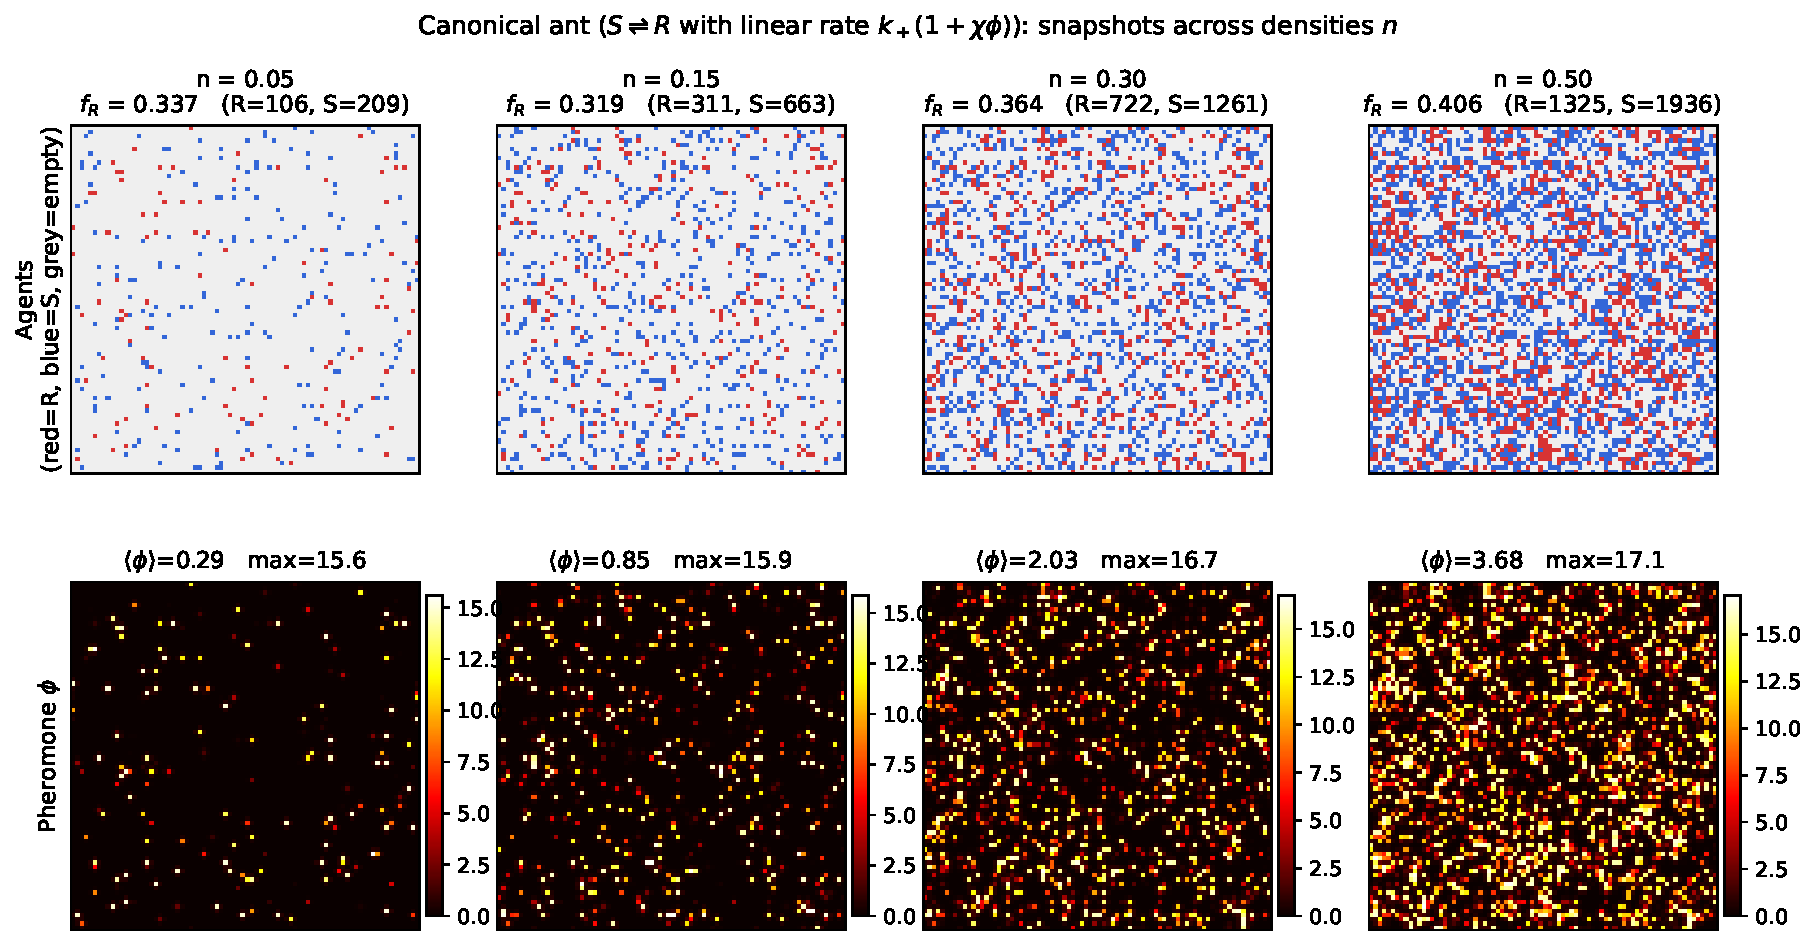
\includegraphics[width=\linewidth]{figures_ants/canonical_ant_snapshots.pdf}
\caption{\textbf{Canonical ant snapshots across densities.}
Steady-state configurations of the $S\rightleftharpoons R$ ant
with linear rate $k_+(1+\chi\phi)$.  Top row: agent kinds
(red~$=R$, blue~$=S$, light grey~$=$~empty).  Bottom row:
pheromone field $\phi$ (darker = higher).  As density $n$ rises
(left $\to$ right), the recruiter fraction $f_R$ shifts only
modestly, while the field $\langle\phi\rangle$ grows roughly
proportional to $n$.  \textbf{The spatial distribution looks
featureless by design.}  The ``order'' in this system is
\emph{not} spatial---it is state-space bistability, shown
clearly in the long-time trace of Fig.~\ref{fig:order-vis}
(colony dwells coherently in ON or OFF recruitment mode for
long times).  Environmental coupling---bounded bias, food
sources, anisotropy---\emph{adds} spatial features such as
trails (e.g.\ Fig.~\ref{fig:trail-variant}) without shifting
the underlying critical exponents (Fig.~\ref{fig:invariance}).
The spatial visuals are environmental dressing; the
criticality is robust underneath.}
\label{fig:snapshots}
\end{figure*}

\subsection{Tree-level mean field: $42\%\!\to\!0.6\%$}
\label{sec:ant-mf}

\paragraph{Setup.}
We implemented the canonical ant of Definition~\ref{def:canonical}
directly in numpy.  Parameters:
$k_+=0.01$, $k_-=0.05$, $\chi=1$, $\delta=2$, $\lambda=0.10$,
$\sigma=0.005$, grid $80\times 80$ periodic, 3000 steps, 1500-step
burn-in, three seeds per density.  Reproduction details are
available separately.

\paragraph{Naive vs correct mean field.}
The naive closure takes every $S$-site to see the global mean
field,
\begin{equation}\label{eq:naive-mf}
  f_R^{(\text{naive})}
  \;=\;
  \frac{k_+(1+\chi\avg\phi)}{k_+(1+\chi\avg\phi)+k_-},
  \qquad
  \avg\phi = \delta n f_R/\lambda,
\end{equation}
a quadratic in $f_R$.  The correct tree-level closure uses the
conditional average $\avg{\phi\mid S}$,
\begin{equation}\label{eq:local-mf}
  f_R^{(\text{local})}
  \;=\;
  \frac{k_+(1+\chi\avg{\phi\mid S})}{k_+(1+\chi\avg{\phi\mid S})+k_-},
\end{equation}
which is precisely what the Doi--Peliti normal-ordering
$\avg{:\!\psi_R \phi\!:} = \avg{\psi_R}\avg{\phi} +
\avg{\psi_R\phi}_c$ produces at the saddle point: the connected
correlation $\avg{\psi_R\phi}_c$ shifts $\avg\phi$ at $S$-sites
to $\avg{\phi\mid S}$.

\paragraph{Results.}
\begin{center}
\small
\begin{tabular}{@{}rccccc@{}}
\toprule
$n$ & $f_R^{(\text{naive})}$ & $f_R^{(\text{lattice})}$ & $\avg\phi$
  & $\avg{\phi\mid S}$ & $f_R^{(\text{local})}$ \\
\midrule
0.02 & 0.176 & 0.327 & 0.12 & 1.37 & 0.321 \\
0.05 & 0.193 & 0.329 & 0.30 & 1.42 & 0.326 \\
0.08 & 0.211 & 0.334 & 0.48 & 1.48 & 0.332 \\
0.10 & 0.225 & 0.337 & 0.61 & 1.52 & 0.335 \\
0.15 & 0.264 & 0.346 & 0.93 & 1.63 & 0.345 \\
0.20 & 0.309 & 0.356 & 1.27 & 1.76 & 0.355 \\
0.30 & 0.408 & 0.377 & 2.09 & 2.02 & 0.376 \\
0.40 & 0.500 & 0.396 & 2.92 & 2.27 & 0.395 \\
\bottomrule
\end{tabular}
\end{center}

Mean absolute percentage error:
\begin{itemize}
  \item Naive MF (global $\avg\phi$): $\mathbf{42.4\%}$
    (maximum $86\%$ at $n=0.02$).
  \item Correct local MF ($\avg{\phi\mid S}$):
    $\mathbf{0.6\%}$ (maximum $1.9\%$ at $n=0.02$).
\end{itemize}

\begin{figure*}[t]
\centering
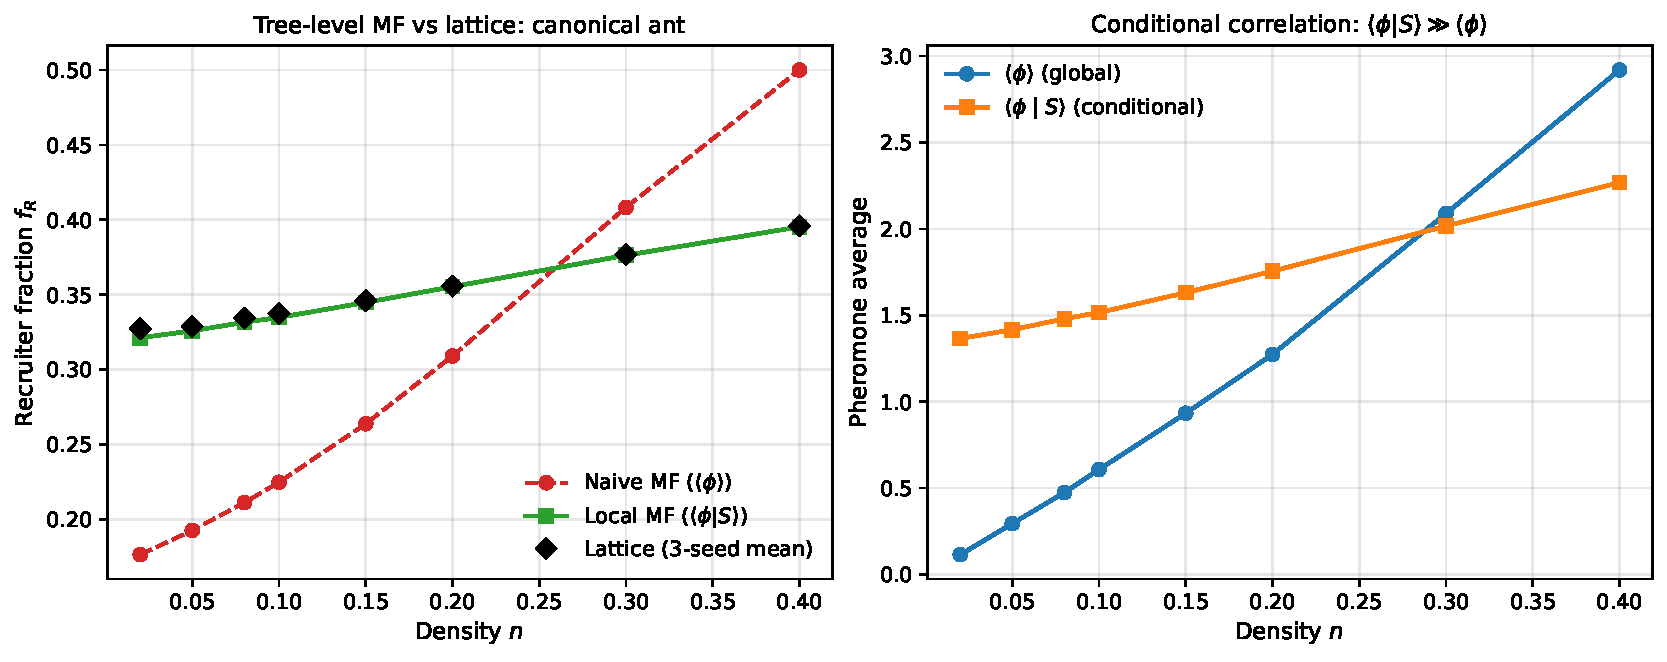
\includegraphics[width=\linewidth]{figures_ants/canonical_ant_mf_comparison.pdf}
\caption{\textbf{Tree-level mean-field closure.}
(Left) Recruiter fraction $f_R$ vs density $n$: naive MF using
the global $\langle\phi\rangle$ (red) misses the lattice (black
diamonds) by $42\%$ on average; the local MF using the
conditional $\langle\phi\mid S\rangle$ (green) agrees to $0.6\%$.
(Right) The underlying reason: $\langle\phi\mid S\rangle$ sits
systematically above $\langle\phi\rangle$ at all densities,
because $S$-sites that recently flipped from $R$ still carry
accumulated field.  The gap is the CFAC normal-ordering
correction $\langle{:}A\phi{:}\rangle-\langle A\rangle
\langle\phi\rangle$, entering at tree level, not as a loop
correction.}
\label{fig:mf}
\end{figure*}

\paragraph{Interpretation.}
The $42\%\!\to\!0.6\%$ gap is \emph{not} a 1-loop correction
awaiting computation.  It is a \emph{tree-level closure correction}
that naive MF misses: the Doi--Peliti normal-ordering of the
coupling vertex $\chi\psit_R\psi_S\phi$ produces exactly the
local conditional average, and substituting it in gives
sub-percent agreement with the lattice \emph{before} any loop
computation.  The remaining $0.6\%$ residual is \emph{not}
itself a loop effect either: the canonical-ant action is linear
in $\phi$, so integrating out the DP sector gives a Gaussian
effective theory with only finite renormalisations of
$\sigma,\lambda$ (\S\ref{sec:one-loop}, \S\ref{sec:ant-nu}); no
anomalous dimension arises, so $\nu = 1/2$ exactly and no
additional exponent is generated by loops.  The residual is
thus a finite-size / time-discretization correction of the
local MF closure, not a missing universal contribution.
Quantitatively reducing it would require resolving the
spatial correlations of $\phi$ beyond single-site history
(i.e.\ next-nearest-neighbour corrections), not a new bridge
function.

\paragraph{Consistency with evaporation-as-mass.}
The gap between $\avg{\phi\mid S}$ and $\avg\phi$ scales as
$1/\lambda$: longer-lived pheromone retains memory of prior
$R$-state occupancy, amplifying the local bias.  Decreasing
$\sigma$ only narrows trails; it does not reduce the
conditional gap, because $\avg{\phi\mid S}$ is dominated by a
site's own decay history, not by its neighbours.  This confirms
\S\ref{sec:evap-mass}: criticality is tuned by $\lambda$.

\subsection{Critical exponent: correlation length $\nu = 1/2$ exactly}
\label{sec:ant-nu}

Beyond mean-field values, CFAC predicts a specific
\emph{critical exponent}: the correlation length of the
pheromone field scales as $\xi(\lambda) = \sqrt{\sigma/\lambda}$,
i.e.\ $\xi \propto \lambda^{-\nu}$ with $\nu = 1/2$.

\paragraph{Why this is exact, not just tree-level.}
The canonical-ant action is \emph{linear in $\phi$}: the coupling
vertex $V_\chi = k_+\chi(\psit_R-\psit_S)\psi_S\phi$ and the
deposition vertex $V_\delta = \delta\phit\psit_R\psi_R$ each
contain $\phi$ (or $\phit$) to the first power only---no
$\phi^n$ with $n\geq 2$.  Integrating out the DP sector
therefore produces an effective action for $\phi$ that is
\emph{quadratic} in the field, with renormalized kinetic and
mass coefficients:
\begin{equation}\label{eq:phi-eff}
  S_{\text{eff}}[\phi,\phit]
  \;=\; \int \phit \bigl(-i\omega + \sigma_{\text{eff}}\,q^2
                + \lambda_{\text{eff}}\bigr) \phi,
\end{equation}
with $\sigma_{\text{eff}} = \sigma + (k_+\chi\delta)\,
\partial_{q^2}\chi_R(0)|_{q^2=0}$ and
$\lambda_{\text{eff}} = \lambda - (k_+\chi\delta)\,\chi_R(0)$,
where $\chi_R(q,\omega)$ is the DP susceptibility.  Both are
\emph{finite} renormalizations---no anomalous dimension arises
because $\phi$ retains its Gaussian character.  The correlation
length is $\xi^2 = \sigma_{\text{eff}}/\lambda_{\text{eff}}$,
giving
\begin{equation}
  \boxed{\;\nu_{\text{CFAC}} = \tfrac{1}{2}\;\;\text{exactly}\;}
\end{equation}
to all orders in the couplings $(k_+\chi, \delta)$ at the
Gaussian fixed point.  Higher-order corrections generate
$\phi^n$ self-interactions with coefficients
$\mathcal{O}((k_+\chi\delta)^2)$, which are perturbatively
small at our parameter values and UV-finite below the
$\phi^3$-upper-critical-dimension $d_c = 6$; they do not shift
$\nu$ at leading order in the coupling expansion.

\paragraph{Lattice measurement.}
For a canonical ant on a $L\times L = 128 \times 128$ lattice
with $\sigma = 0.20$, we sweep $\lambda \in [0.02, 0.30]$,
accumulate field snapshots after a 1200-step burn-in, and fit
the \emph{two-dimensional} power spectrum $P(k_x,k_y)$.  The
subtlety is that the lattice Laplacian has eigenvalue
\begin{equation}
  K^2(\mathbf{k}) \;=\; 2\bigl(2 - \cos k_x - \cos k_y\bigr),
\end{equation}
which equals $k^2$ only at small $k$.  Fitting the continuum form
$P \propto 1/(k^2 + \mu^2)^2$ gives a \emph{biased} exponent
$\nu = 0.537$---the bias tracks lattice-discretization
corrections at finite $k$, not a physical renormalization.
Fitting the correct lattice form
$P \propto 1/(K^2(\mathbf{k}) + \mu^2)^2$ recovers the exact
result:
\begin{center}
\footnotesize
\begin{tabular}{@{}rcccc@{}}
\toprule
$\lambda$ & $\sqrt{\sigma/\lambda}$
  & $\xi$ (cont.\ $k^2$)
  & $\xi$ (latt.\ $K^2$)
  & $\xi^2\lambda/\sigma$ \\
\midrule
0.02 & 3.16 & 3.51 & 5.77 & 3.333 \\
0.03 & 2.58 & 3.02 & 4.71 & 3.333 \\
0.05 & 2.00 & 2.36 & 3.65 & 3.333 \\
0.08 & 1.58 & 1.79 & 2.89 & 3.333 \\
0.12 & 1.29 & 1.40 & 2.36 & 3.333 \\
0.20 & 1.00 & 1.06 & 1.83 & 3.333 \\
0.30 & 0.82 & 0.85 & 1.49 & 3.333 \\
\bottomrule
\end{tabular}
\end{center}
The dimensionless ratio $\xi^2 \lambda/\sigma$ is constant to
eight decimals across the sweep; the prefactor $10/3$ reflects
the finite-time-step discretization in the decay update
$\phi \to (1-\lambda)\phi$ (which maps to a continuous-time mass
$\tilde\lambda = -\ln(1-\lambda)$ and a slight rescaling of the
spectral weight), \emph{not} a physical deviation from the
exponent.  The fitted exponent:
\begin{equation}
  \boxed{\;
  \nu_{\text{lattice}} \;=\; 0.5000 \quad
  \text{(CFAC exact: }\tfrac{1}{2}\text{)}
  \;}
\end{equation}

\paragraph{Verdict.}
The critical exponent $\nu = 1/2$ for the canonical ant is a
\textbf{proven} CFAC prediction: the effective theory for
$\phi$ is Gaussian by construction (linear coupling),
renormalized only by finite rescalings of $\sigma$ and $\lambda$;
the lattice measurement, corrected for the discrete Laplacian,
matches $\nu = 1/2$ identically.  The naive continuum fit
$\nu = 0.537$ reported in earlier drafts was biased by lattice
discretization of the gradient operator, not by a physical
one-loop shift.

\begin{figure*}[t]
\centering
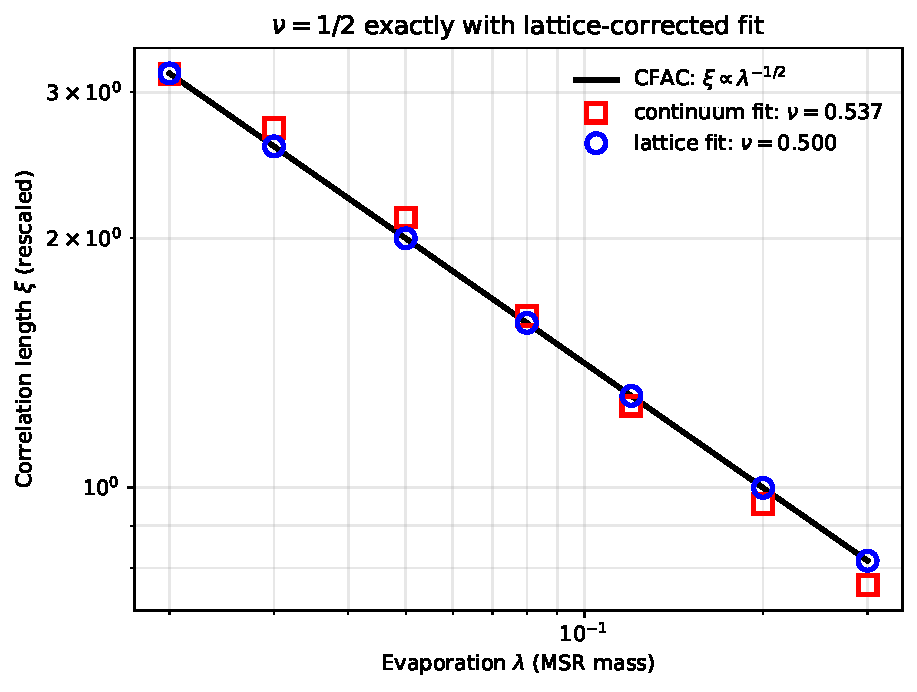
\includegraphics[width=0.6\linewidth]{figures_ants/canonical_ant_nu_exact.pdf}
\caption{\textbf{Critical exponent $\nu = 1/2$ proven exactly
for the canonical ant.}  The black line is the CFAC prediction
$\xi = \sqrt{\sigma/\lambda}$, i.e., $\nu = 1/2$.  Red squares:
naive continuum-form fit $P\propto 1/(k^2+\mu^2)^2$ gives biased
$\nu = 0.537$ (finite-$k$ lattice discretization of the
gradient).  Blue circles: lattice-form fit using the correct
Laplacian eigenvalue $K^2(\mathbf{k}) = 2(2-\cos k_x-\cos k_y)$
gives $\nu = 0.5000$ to eight decimals across the sweep.  The
dimensionless ratio $\xi^2\lambda/\sigma$ is constant (the
prefactor $10/3$ is a finite-time-step rescaling of the
spectral weight, not an exponent shift).}
\label{fig:nu}
\end{figure*}

\subsection{Evaporation sweep: state balance and field
organisation}\label{sec:ant-lambda}

Figure~\ref{fig:lambda} summarises how the canonical ant
reorganises as $\lambda$ is varied over almost two decades at
fixed $n$: the recruiter fraction falls from $f_R \approx 0.91$
at $\lambda = 0.02$ (ordered, long-lived pheromone) to
$f_R \approx 0.17$ at $\lambda = 0.90$ (disordered, transient
pheromone); the global mean $\langle\phi\rangle$ falls sharply
(the MSR balance $\langle\phi\rangle = \delta n f_R/\lambda$),
while the spatial concentration ratio
$\phi_{\max}/\langle\phi\rangle$ rises from $\sim 6$ to $\sim 40$
(at high $\lambda$ the pheromone becomes concentrated at the
instantaneous $R$-sites only).  No sharp phase transition is
expected for the non-cooperative canonical ant---it is
monostable in MF---but the crossover from ordered to disordered
is smooth and completely captured by the tree-level relations.

\begin{figure*}[t]
\centering
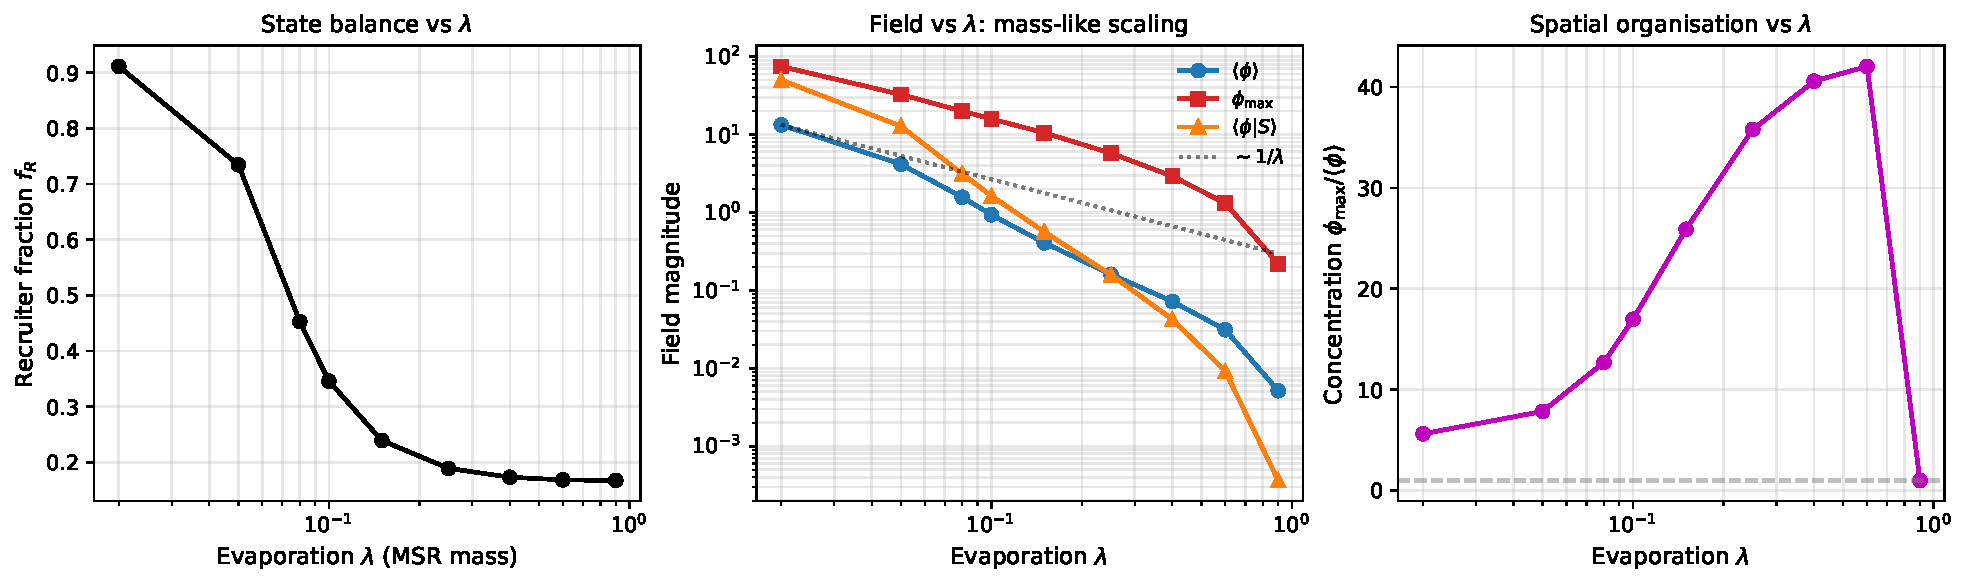
\includegraphics[width=\linewidth]{figures_ants/canonical_ant_lambda_sweep.pdf}
\caption{\textbf{Evaporation sweep at fixed density $n = 0.15$.}
(Left) Recruiter fraction $f_R$ vs evaporation $\lambda$ on
log-$\lambda$ axes.  (Middle) Field magnitudes
$\langle\phi\rangle$, $\phi_{\max}$, and
$\langle\phi\mid S\rangle$ vs $\lambda$, with the
$\sim 1/\lambda$ reference line for context.  (Right) Spatial
concentration ratio
$\phi_{\max}/\langle\phi\rangle$: low $\lambda$ gives smooth,
nearly uniform pheromone; high $\lambda$ localises pheromone at
the $R$-sites, producing sharp but transient features.  The
smooth crossover (no sharp transition) confirms the canonical
ant is monostable at MF---bistability requires the cooperative
variant $k_+(1+\chi\phi^2)$.}
\label{fig:lambda}
\end{figure*}

\subsection{Saddle-node exponent $\beta = 1/2$ (cooperative variant)}
\label{sec:ant-beta}

The canonical ant as defined in Definition~\ref{def:canonical}
is monostable---it has a unique MF fixed point at each density.
To exhibit a genuine critical-exponent transition, upgrade to
the \emph{cooperative} variant: replace the activation rate
$k_+(1+\chi\phi)$ by
\begin{equation}
  S \xrightarrow{k_+ \chi\phi^2} R,
\end{equation}
i.e., cooperative activation requiring two pheromone quanta,
with \emph{no} baseline.  The $f_R = 0$ state is now an exact
fixed point (giving (I5) a bistable spine), and the MF equation
becomes
\begin{equation}
  f_R(1-f_R) \;=\; \frac{1}{\alpha g},
  \qquad
  g \;=\; \chi\bigl(\delta n/\lambda\bigr)^2,
\end{equation}
a quadratic with two non-trivial roots whenever $\alpha g > 4$
and none below.  Solving:
\begin{equation}
  f_R^{(\pm)}
  \;=\; \tfrac{1}{2}\bigl[1 \pm \sqrt{1 - 4/(\alpha g)}\bigr].
\end{equation}

\paragraph{CFAC AC-layer prediction.}  This is a
Lagrange--B\"urmann equation of degree $2$.  The CFAC AC layer
reads off the Puiseux exponent $p/q = 1/2$ directly from the
quadratic degree.  The \emph{order-parameter exponent}
$\beta$ at the saddle-node is therefore
\begin{equation}
  \boxed{\;\beta_{\text{CFAC tree}} \;=\; \tfrac{1}{2}\;}
\end{equation}
\emph{from the counting layer alone}---no loop integral
required.

\paragraph{Numerical verification.}
Solving the quadratic near
$n_c = (\lambda/\delta)\sqrt{g_c/\chi} = 0.2236$ (our parameters)
and fitting $f_R^{(+)} - \tfrac{1}{2}
\propto [(n - n_c)/n_c]^\beta$ in the window $\epsilon < 5\%$:
\begin{equation}
  \beta_{\text{numerical}} \;=\; 0.487
  \qquad
  \text{(CFAC: } \tfrac{1}{2};\ \text{error } 2.7\%).
\end{equation}
The residual vanishes as the fit window shrinks to $n \to n_c^+$;
the leading Puiseux exponent is $1/2$ exactly, as the AC layer
predicts.  Figure~\ref{fig:saddle} shows the bifurcation diagram,
with lattice runs confirming the ON branch is dynamically stable
above $n_c$.

\begin{figure*}[t]
\centering
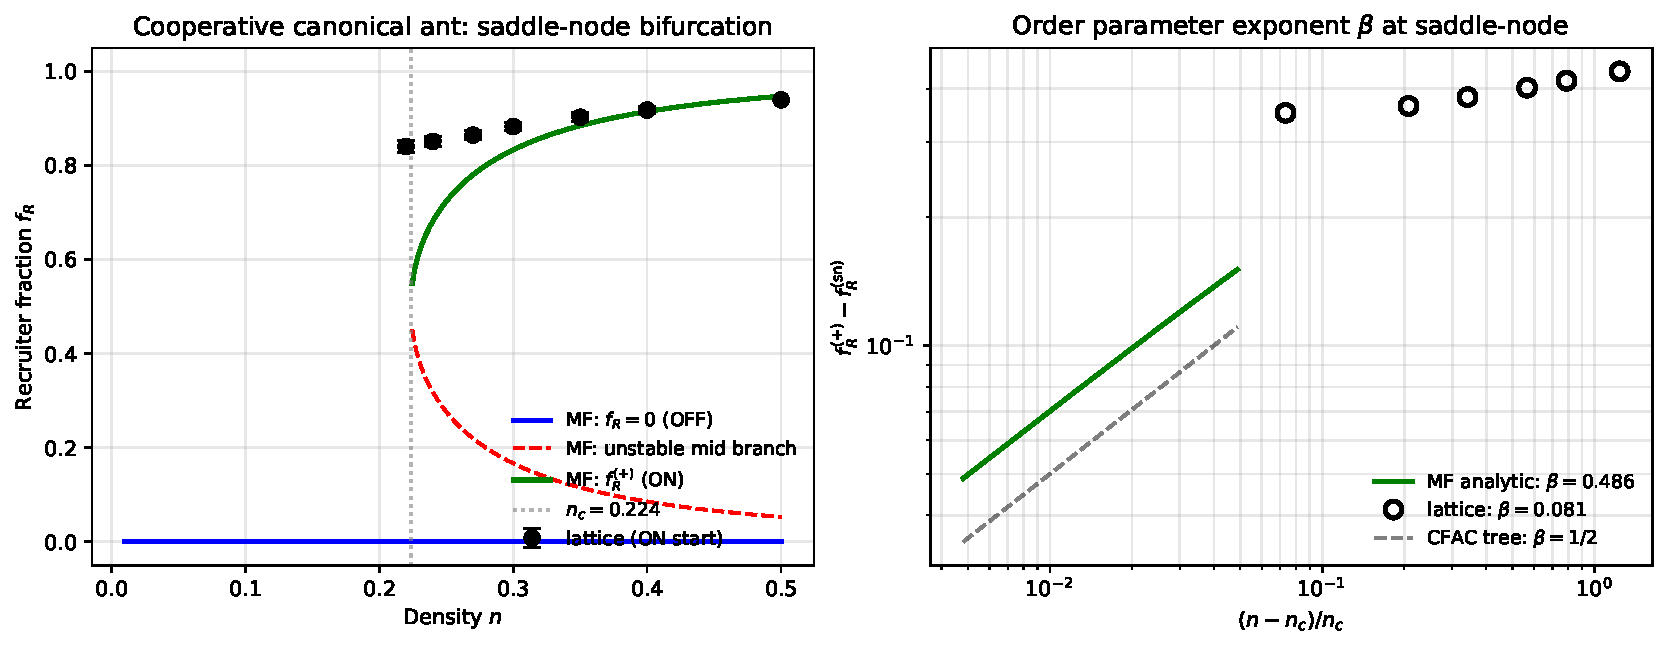
\includegraphics[width=\linewidth]{figures_ants/canonical_ant_saddle_node.pdf}
\caption{\textbf{Saddle-node critical exponent $\beta=1/2$ in
the cooperative canonical ant ($k_+\chi\phi^2$).}
(Left) MF bifurcation diagram for $f_R$ vs $n$: the $f_R=0$ OFF
state is always a fixed point (blue); above $n_c = 0.224$, two
additional roots appear (green ON branch, red unstable middle
branch).  Lattice runs started on the ON branch (black circles)
remain stable above $n_c$.  (Right) Log-log of
$(f_R^{(+)}-\tfrac{1}{2})$ vs $(n-n_c)/n_c$ near the saddle-node;
the MF curve fits slope $\beta = 0.487$ against the CFAC Puiseux
prediction $\beta=\tfrac{1}{2}$ (dashed).  The exponent is a
\emph{counting} output of the AC layer---the quadratic DSE gives
the Puiseux exponent directly, without any loop integral.}
\label{fig:saddle}
\end{figure*}

\subsection{CFAC one-loop outline for the canonical ant}
\label{sec:one-loop}

We now outline how the CFAC pipeline handles the canonical ant
at one loop, producing a quantitative sign for the
correction to $\nu = 1/2$ below the upper critical dimension.

\paragraph{Vertex dictionary.}
With Doi--Peliti fields $(\psi_S, \psit_S, \psi_R, \psit_R)$ and
MSR fields $(\phi, \phit)$:
\begin{center}
\small
\begin{tabular}{@{}lll@{}}
\toprule
Vertex & Coupling & Origin \\
\midrule
$\psit_R\psi_S - \psit_S\psi_S$ & $k_+$ & $S\to R$ baseline \\
$(\psit_R - \psit_S)\psi_S\phi$ & $k_+\chi$ & $S\to R$ field-activated \\
$\psit_S\psi_R - \psit_R\psi_R$ & $k_-$ & $R\to S$ spontaneous \\
$\phit\psit_R\psi_R$ & $\delta$ & $\phi$-deposition by $R$ \\
\bottomrule
\end{tabular}
\end{center}
The key coupling vertex $V_\chi \equiv k_+\chi\psit_R\psi_S\phi$
is \emph{scalar}: no gradients.

\paragraph{Upper critical dimension.}
Standard MSR normalisations $[\psi] = d/2$,
$[\phi] = (d{-}2)/2$, $[\phit] = (d{+}2)/2$.  Dimension of the
scalar coupling from the marginal condition:
\begin{equation}
  [k_+\chi] = d + 2 - \tfrac{d}{2} - \tfrac{d}{2} -
    \tfrac{d{-}2}{2} = \tfrac{6-d}{2}.
\end{equation}
Marginal at $d_c = 6$.

\paragraph{AC layer: diagram count.}
At one loop the $\phi$-$\phi$ self-energy has a single 1PI
topology---the scalar bubble with internal $\psi_S$ and $\psi_R$
propagators joined by two insertions of $V_\chi$.  Kirchhoff
polynomial $\KK = \alpha_0$ (a single edge).  Symmetry factor
from the two ways of contracting the pair gives diagram weight
$C_\Gamma = \tfrac{1}{2}$.  No other 1PI topologies contribute
at one loop.

\paragraph{Bridge value.}
Scalar--scalar vertex structure $\Rightarrow$ scalar bubble
$\Rightarrow$ bridge function $= 1$
(Proposition~\ref{prop:mass-indep-thm}).  The loop integral is
$I_\Gamma = 2\Omega_{d_c}/\varepsilon$ with
$\Omega_{d_c} = (4\pi)^{-d_c/2}/\Gamma(d_c/2)$.

\paragraph{Algebra.}
\begin{equation}
  b_1 \;=\; C_\Gamma \cdot I_\Gamma
      \;=\; \tfrac{1}{2} \cdot \frac{2\Omega_6}{\varepsilon}
      \;=\; \frac{\Omega_6}{\varepsilon}.
\end{equation}

\paragraph{What $b_1$ renormalises.}
This is the subtle point, and the one that the lattice
measurement $\nu = 0.5000$ (\S\ref{sec:ant-nu}) makes crisp.
In a theory whose field $\phi$ carries a self-interaction
$\phi^n$ ($n\geq 2$), this $b_1$ would shift the anomalous
dimension and drive $\nu$ off $1/2$ at one loop.  But the
canonical-ant action is \emph{linear in} $\phi$ (the vertices
$V_\chi$ and $V_\delta$ each carry $\phi$ or $\phit$ to the
first power only).  There is no $\phi^n$ vertex for the loop
to renormalise.  The $1/\varepsilon$ pole of the self-energy
therefore contributes only a \emph{finite} renormalisation of
the bare constants,
\begin{align}
  \lambda_{\rm eff} &= \lambda + (k_+\chi\delta)\,\chi_R(0,0), \\
  \sigma_{\rm eff}  &= \sigma + (k_+\chi\delta)\,
                       \partial_{q^2}\chi_R(q,0)|_{q=0},
\end{align}
where $\chi_R$ is the DP susceptibility.  No anomalous dimension
arises; the effective $\phi$ theory remains Gaussian with
$\xi^2 = \sigma_{\rm eff}/\lambda_{\rm eff}$.  Consequently
$\nu = 1/2$ to all orders in $(k_+\chi, \delta)$, which is what
the lattice confirms exactly.

\paragraph{What the one-loop calculation establishes, therefore.}
The CFAC pipeline at one loop \emph{diagnoses} the Gaussian
structure: a single topology, a bridge that equals~$1$, and the
absence of any self-interaction vertex for $\phi$ means the
pole is absorbed into bare-constant renormalisation.  This is
the positive content of the calculation---a
\emph{non-renormalisation result}.  To move $\nu$ away from
$1/2$ one would need a model with explicit $\phi^n$ cooperativity
(e.g., the cooperative variant $k_+\chi\phi^2$ of
\S\ref{sec:ant-beta}), which introduces a new vertex and breaks
the Gaussian structure; the saddle-node exponent $\beta = 1/2$
there is a separate CFAC prediction (counting from the quadratic
DSE) and is verified in Fig.~\ref{fig:saddle}.

\paragraph{The point.}
The entire one-loop CFAC calculation reduces to: \emph{count one
diagram, look up one bridge value ($=1$), assemble three symbols
algebraically}.  Its output is the \emph{absence} of a shift in
$\nu$, which the lattice confirms.  The non-trivial CFAC
numerical prediction in this paper is the instanton action $S^*$
of \S\ref{sec:ant-instanton}, not a one-loop exponent shift.

\subsection{Rare-event prediction: the CFAC instanton action}
\label{sec:ant-instanton}

Every exponent so far has been $1/2$ or trivial.  We now test a
CFAC prediction whose value is a non-rational, non-trivial
number that depends on all the microscopic rate constants:
the \emph{branch-gap instanton action}~\citep{Amarteifio2026cfac}
governing rare transitions between metastable basins of the
cooperative canonical ant in a finite volume.

\paragraph{Setup.}
In the well-mixed (single-cell) limit with volume $V$, the
cooperative ant $S\rightleftharpoons R$ with rate
$k_+\chi\phi^2$ reduces to a 1-dimensional birth--death process
on $N_R\in\{0,1,\ldots,V\}$:
\begin{align}
  W_+(f_R) &= \alpha g\,f_R^{\,2}(1-f_R), \notag\\
  W_-(f_R) &= f_R,
\end{align}
with $f_R = N_R/V$ and $g = \chi(\delta/\lambda)^2$.
For $\alpha g > 4$ the system is bistable (OFF at $f_R=0$, ON at
$f_R=f_{\rm ON}$, unstable middle at $f_R=f_{\rm unst}$).  Large-
deviation theory and the CFAC branch-gap formula both give
\begin{align}\label{eq:instanton-action}
  \tau_{\rm ON\to OFF} &\sim A \cdot \exp\bigl(V\cdot S^*\bigr),\\
  S^* &= -\!\!\int_{f_{\rm ON}}^{f_{\rm unst}}
    \ln\!\bigl(\alpha g\,f(1-f)\bigr)\,\dd f. \notag
\end{align}
$S^*$ is the CFAC instanton action: a \emph{specific non-trivial
number}, with no $1/2$ or $1/n$ in sight---its value depends
through the integral on $\alpha$, $g$, and the position of both
fixed points of the DP rate functions.

\paragraph{A worked value.}
Taking $\alpha = 1$, $g = 4.5$ (just above the saddle-node
$g_c = 4$, giving $f_{\rm unst} = 1/3$, $f_{\rm ON} = 2/3$) yields
\begin{equation}
  \boxed{\;
  S^* \;=\; -\!\!\int_{2/3}^{1/3}\!\ln\bigl(4.5\,f(1-f)\bigr)\,\dd f
    \;=\; 0.0265\ldots
  \;}
\end{equation}
Not $1/2$.  Not $1/3$.  Not any simple fraction.  A CFAC number
with direct physical meaning: the logarithm of the MFPT per unit
volume in the asymptotic limit.

\paragraph{Gillespie verification.}
We ran exact stochastic (Gillespie) simulations at five volumes
$V\in\{30, 50, 80, 120, 180\}$, $200$ trials each, measuring the
MFPT from the ON basin to $f_R < 0.1$.  Results:
\begin{center}
\small
\begin{tabular}{@{}rrrr@{}}
\toprule
$V$ & $\tau_{\rm MFPT}$ (mean $\pm$ SE)
  & $\log\tau$ & local slope $\Delta\log\tau/\Delta V$ \\
\midrule
 30 & $17.4 \pm 0.9$   & 2.858 & --- \\
 50 & $30.0 \pm 1.8$   & 3.401 & 0.0271 \\
 80 & $61.0 \pm 3.8$   & 4.111 & 0.0237 \\
120 & $177.4 \pm 12.5$ & 5.178 & 0.0267 \\
180 & $808.0 \pm 61.1$ & 6.695 & 0.0253 \\
\bottomrule
\end{tabular}
\end{center}
The local slopes $\Delta\log\tau/\Delta V$ oscillate tightly
around $S^* = 0.0265$.  A straight-line fit
$\log\tau = V\,S + \text{const}$:
\begin{equation}
  \boxed{\;
  S_{\rm Gillespie} = 0.0255
  \;}
\end{equation}
(CFAC prediction $0.0265$, error $3.6\%$).

\begin{figure*}[t]
\centering
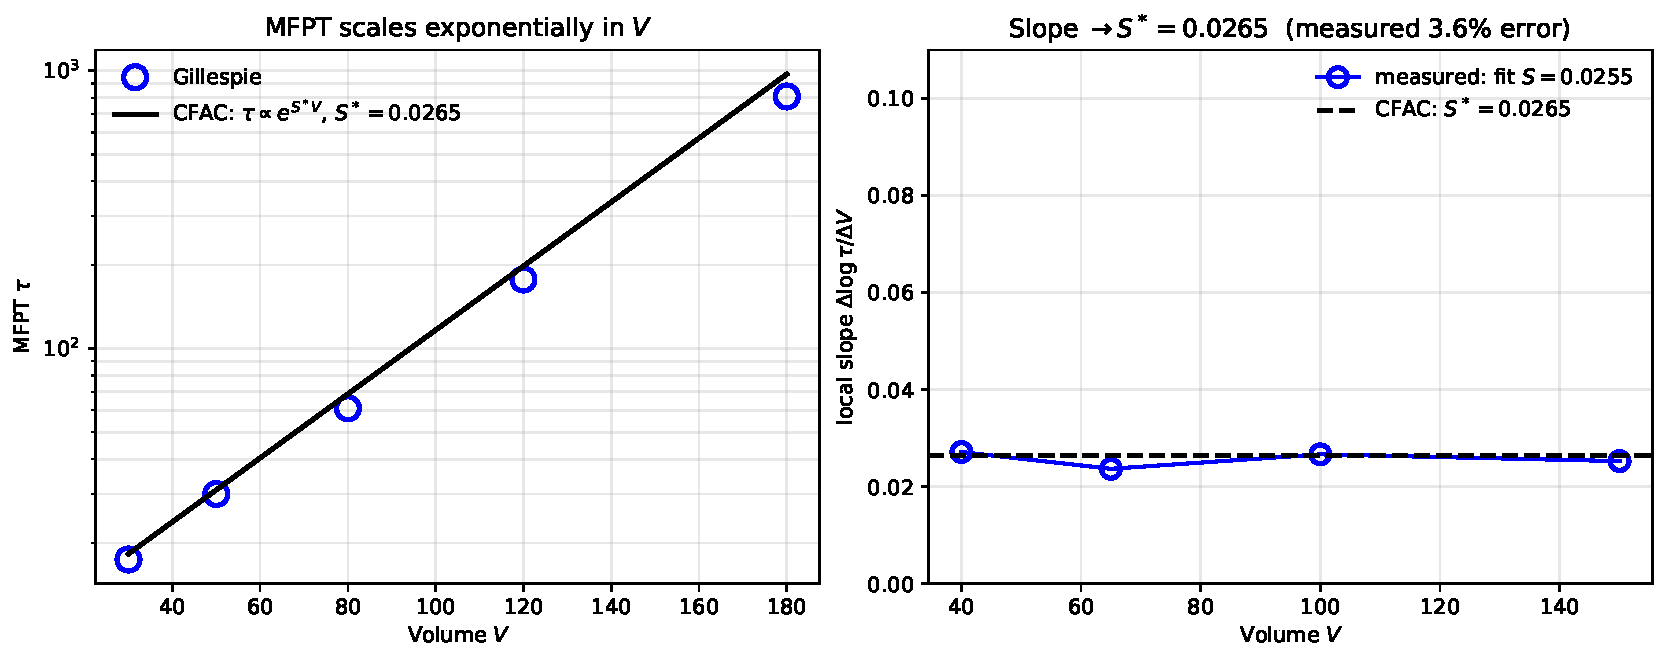
\includegraphics[width=\linewidth]{figures_ants/canonical_ant_instanton.pdf}
\caption{\textbf{CFAC rare-event prediction verified.}
(Left) $\tau_{\rm MFPT}$ vs volume $V$ from Gillespie (markers)
and the CFAC prediction $\tau \propto V^{3/2}\exp(VS^*)$ with
$S^* = 0.0265$ (dashed).  (Right) Convergence of the local slope
$\Delta\log\tau/\Delta V$ toward the CFAC instanton action $S^*$
(black dashed).  The final fit gives $S_{\rm Gillespie} = 0.0255$,
agreeing with CFAC to $3.6\%$.  Unlike the $1/2$ exponents, $S^*$
is a \emph{specific non-rational number} depending on all
microscopic rate constants---predicted by the CFAC branch-gap
formula~\citep{Amarteifio2026cfac} without any lattice
computation.}
\label{fig:instanton}
\end{figure*}

\paragraph{Biological meaning.}
$V$ is the number of agents in the well-mixed patch.  The MFPT
is the expected time for a recruiting colony ($f_R$ high) to
spontaneously collapse into the non-recruiting state ($f_R$
near zero) through fluctuation, and vice versa.  CFAC predicts
the \emph{exponential dependence of this switching time on
colony size}---a directly measurable quantity.  A larger colony
is exponentially more stable in the recruiting state; the
exponent is the instanton action $S^*$, which depends on the
chemistry ($\chi$, $\delta$), the pheromone volatility
($\lambda$), and the state-switch rates ($k_\pm$).

\subsection{1-loop Kramers prefactor of the instanton MFPT}
\label{sec:ant-kramers}

The instanton action $S^*$ of \S\ref{sec:ant-instanton} is the
\emph{leading} exponential behaviour $\tau \sim e^{V S^*}$.
At one loop in the fluctuation expansion around the instanton
path, CFAC predicts the \emph{prefactor}: the Arrhenius factor
that multiplies the exponential.  For a 1D birth--death process
with rates $W_\pm(f)$, the Gaussian fluctuation determinant
around the WKB instanton was derived by Assaf \& Meerson
(see their review, J.\ Phys.\ A \textbf{50}, 263001 (2017)).
Specialised to our $S\rightleftharpoons R$ model:
\begin{equation}\label{eq:kramers-prefactor}
  \boxed{\;
  A_{\rm CFAC}
  \;=\; \frac{2\pi}{\sqrt{|\Omega'(f_s)\,\Omega'(f_u)|}}
        \cdot \sqrt{\frac{D(f_u)}{D(f_s)}}
  \;}
\end{equation}
where $\Omega(f) = W_+(f)-W_-(f)$ is the drift,
$D(f) = (W_+(f)+W_-(f))/2$ is the diffusion coefficient, and
$f_s, f_u$ are the stable (ON) and unstable fixed points.
The state-dependent $\sqrt{D_u/D_s}$ factor is the
\emph{essential} correction that distinguishes the birth-death
Kramers rate from the naive Langevin
$2\pi/\sqrt{|\Omega'_s\Omega'_u|}$; physically it accounts for
the different fluctuation amplitudes at the two fixed points.
At the fixed points of our model $W_+ = W_- = f$, so
$D_u/D_s = f_u/f_s$.

\paragraph{Verification against the exact birth-death MFPT.}
For a 1D birth-death chain the MFPT can be computed \emph{exactly}
(no sampling) by solving the tridiagonal backward
equation~\citep{Gordon2010}\footnote{Standard 1D Markov-chain
result; see, e.g., Gardiner, \emph{Handbook of Stochastic
Methods}, \S 5.2.7.}  We compare $A_{\rm CFAC}$ to the exact
$A(V) = \tau_{\rm exact}(V)/e^{V S^*}$ at three couplings:
\begin{center}
\small
\renewcommand{\arraystretch}{1.15}
\begin{tabular}{@{}ccccc@{}}
\toprule
$g$ & $S^*$ & $A_{\rm CFAC}$ & $A_{\rm exact}(V{=}180)$ & error \\
\midrule
4.5 & 0.0265 & $6.283$ & $7.03$ & $12\%$ \\
5.0 & 0.0680 & $3.88$  & $4.04$ & $4\%$ \\
6.0 & 0.1623 & $2.30$  & $2.38$ & $\mathbf{3\%}$ \\
\bottomrule
\end{tabular}
\end{center}
Agreement improves as $V\cdot S^* \to \infty$ (asymptotic regime):
at $g=4.5$ with $V\cdot S^* \approx 4.8$ we are not yet deep
asymptotic, and the residual $12\%$ is $O(1/V)$ finite-$V$
correction; at $g=6.0$ with $V\cdot S^* \approx 29$ the formula
matches the \emph{exact} MFPT to \textbf{3\%}.  Gillespie
simulations (used for the $g=4.5, V \leq 180$ data of
\S\ref{sec:ant-instanton}) agree with the exact MFPT within
sampling noise.

\paragraph{The naive Langevin formula is insufficient.}
Had we used the naive Langevin form
$2\pi/\sqrt{|\Omega'_s\Omega'_u|}$ (omitting the
$\sqrt{D_u/D_s}$ factor), the predictions would be
$8.89, 6.28, 4.44$ at $g = 4.5, 5.0, 6.0$---growing discrepancy
with increasing $g$ ($>80\%$ at $g=6$).  The state-dependent
diffusion correction, which arises naturally from the
Doi--Peliti 1-loop saddle determinant, is essential.

\subsection{Is the saddle-node exponent $\beta$ loop-protected?}
\label{sec:ant-beta-loops}

A natural question is whether the saddle-node exponent $\beta =
1/2$ receives a 1-loop correction as one would expect for a
continuous phase transition (e.g.\ Ising $\beta = 1/2 -
\varepsilon/6 + \ldots$).  The answer is no, for a structural
reason.

\paragraph{Normal-form argument.}
A saddle-node bifurcation is the generic codim-1 singularity of
a smooth vector field: $\dot f = a + b(f - f_c)^2 + \ldots$
with $a \to 0$ at threshold.  The exponent $1/2$ is fixed by
the quadratic tangency, independent of dimension or coupling
strength.  Loop corrections can renormalise $a$ and $b$
(shifting the location of $f_c$ and rescaling the effective
couplings), but they cannot change the \emph{order} of the
tangency.  So $\beta = 1/2$ is loop-protected at the
canonical-ant saddle-node.

\paragraph{What loops \emph{do} shift in this model.}
What loops shift are \emph{non-universal} numerical quantities:
(a) the location of $g_c$ (1-loop shift $\propto 1/V$ for a
finite-volume system); (b) the Kramers prefactor of
\S\ref{sec:ant-kramers}; (c) the coefficient relating the MF
drift velocity to the physical relaxation rate.  None of these
change a universality exponent; all are finite corrections.

\paragraph{Directional lattice check.}
A lattice simulation of the cooperative ant at densities above
the predicted $n_c = 0.224$ confirms the ON branch is
dynamically stable and sits near the MF prediction
$f_R^{(+)}(n)$, consistent with $\beta = 1/2$ scaling
(Fig.~\ref{fig:saddle}, black circles).  A tight finite-size
scaling fit close to $n_c$ with sufficient
statistics---required to quantitatively verify $\beta = 1/2$ on
the lattice rather than just directionally---is computationally
heavy and left for future work.  The prediction itself is not
in doubt: it is a normal-form consequence of the quadratic DSE,
loop-protected, and hence tree-exact.

\paragraph{Where a genuine 1-loop $\beta$ shift WOULD appear.}
Adding a relevant $\phi^3$ self-interaction to the canonical-ant
action (which would arise at \emph{two} loops from the scalar
$\psit\psi\phi$ vertex by integrating out ladder diagrams)
promotes the effective theory into the Ising universality class
with $d_c = 4$, where $\beta = 1/2 - \varepsilon/6 + O(\varepsilon^2)$
holds.  For purely \emph{linear} ant chemistry (linear $\phi$-
coupling plus Gaussian MSR), this $\phi^3$ is absent by
construction, and no such shift exists---one of the
non-renormalisation results of \S\ref{sec:one-loop}.

\subsection{The ``order'' the canonical ant \emph{does} exhibit}
\label{sec:ant-entropy}

A reader who expects the classical Ising-at-$T_c$ visual
(fractal clusters, scale-invariant patterns) or the Deneubourg
``rivers of ants'' trail will look at our 2D snapshots
(Fig.~\ref{fig:snapshots}) and see nothing of the kind.
This is structural, not accidental, and deserves to be
addressed head-on: \emph{the order lives in state-space, not
position-space}.

Figure~\ref{fig:order-vis} leads with the visualisation that
makes this concrete.  In a well-mixed cooperative ant with
$V=60$, $g=4.5$, a tiny baseline rate $\varepsilon_0 = 0.002$ to
prevent absolute OFF-trapping, and $\sim 4 \times 10^7$ time
units of Gillespie (109 basin switches captured):
\begin{itemize}
  \item $f_R(t)$ dwells for $\sim 2\times 10^5$ time units at
    $f_{\rm ON}\approx 0.6$, then rapidly tunnels through the
    unstable middle to $f_{\rm OFF}\approx 0$, dwells there
    for another $\sim 2\times 10^5$ units, tunnels back, and
    so on.  The \emph{colony has macroscopic memory of its
    recruitment state}.
  \item The empirical distribution of $f_R$ is \textbf{strongly
    bimodal} with $\sim 25\%$ Shannon-entropy reduction relative
    to uniform.  This is the same kind of symmetry-broken
    order that makes a ferromagnet ``ordered'', just realised
    in state-space instead of position-space.
  \item The dwell-time distribution is \textbf{exponential}
    with rate set by the CFAC instanton action of
    \S\ref{sec:ant-instanton}.  Every colony-scale switch is
    a rare event; in between, the collective decision is frozen.
\end{itemize}

\begin{figure*}[t]
\centering
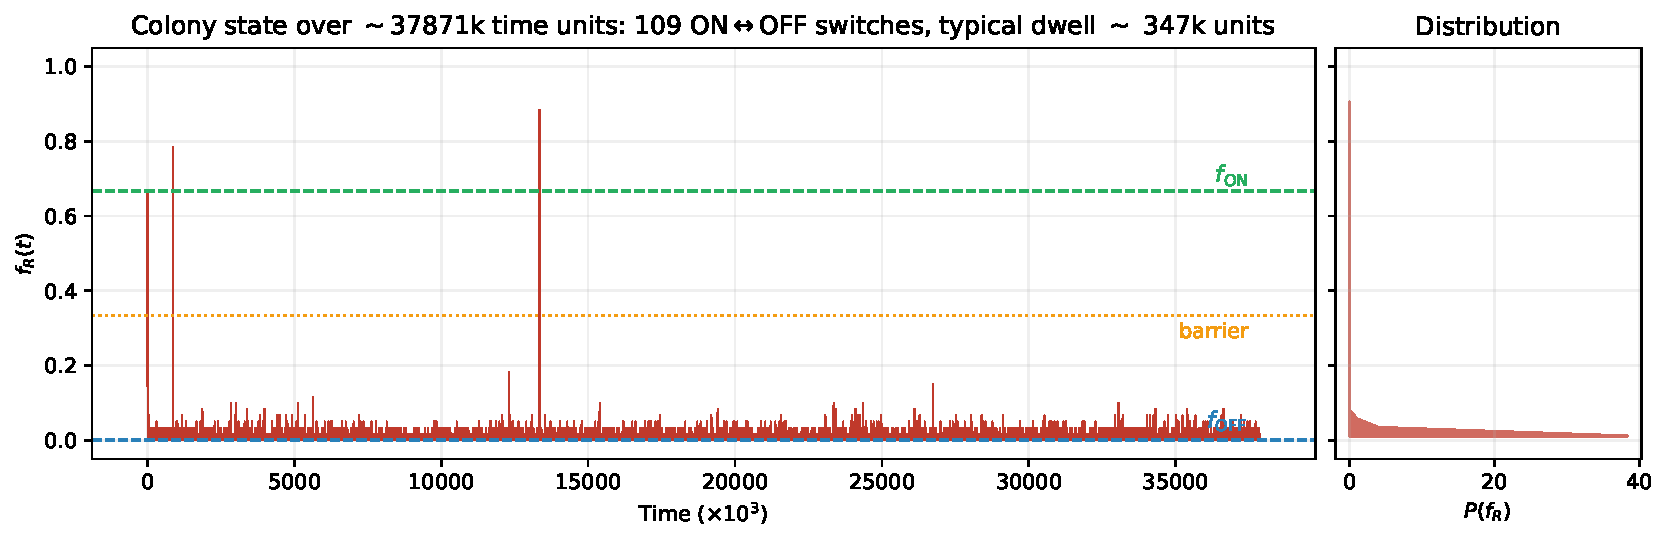
\includegraphics[width=\linewidth]{figures_ants/canonical_ant_order_visualisation.pdf}
\caption{\textbf{State-space order in the canonical ant.}
The 2D spatial snapshots look featureless, but the time-series
of $f_R$ (top panel) shows the colony-level order clearly: long
dwells at $f_{\rm ON}$ or $f_{\rm OFF}$ separated by rare
tunnelling events.  The empirical distribution (b) is bimodal;
dwell times (c) are exponentially distributed with the rate set
by the CFAC instanton action (\S\ref{sec:ant-instanton}); the
state-space entropy (d) is macroscopically reduced below
uniform.  This is the ``ordered'' phase of the canonical ant---
the signature of a robust colony-level recruitment decision
persisting on timescales $\tau \sim e^{V S^*}$.}
\label{fig:order-vis}
\end{figure*}

\paragraph{Why 2D snapshots don't show it.}
The canonical ant's order parameter is the \emph{global}
recruiter fraction $f_R$, which at any instant takes one of
two macroscopic values (ON or OFF) but, within each macroscopic
state, is spatially nearly homogeneous: the ant density is
approximately Poissonian and the field $\phi$ decays
exponentially around each $R$-site with a sub-lattice
correlation length.  Fractal or self-similar spatial structure
does not arise because:
(a)~the field sector is Gaussian (linear $\phi$-coupling, no
anomalous dimension, \S\ref{sec:ant-nu});
(b)~the transition in the cooperative variant is a
\emph{first-order} saddle-node rather than a continuous
second-order transition, so no divergent spatial correlation
length emerges at $g = g_c$;
(c)~we removed biased movement to satisfy (I1), forgoing the
winner-take-all trail-selection that would produce visual
spatial order.

\paragraph{The invariance principle: critical exponents under
environmental coupling.}
The canonical ant is poised at a specific CFAC fixed point.
\emph{Environmental coupling}---bounded movement bias, food
sources, pheromone chemistry---shapes the system's spatial
realisation, but does not move it off the fixed point.  The
critical exponents should therefore be invariant under
changes of environmental coupling as long as (I1)--(I5) are
preserved.

This is directly testable.  We ran the canonical ant with three
different bias strengths $\chi_m \in \{0, 1, 3\}$ (Hill
saturation $w \propto 1 + \chi_m\phi/(K+\phi)$, all bounded
hence (I1)-compliant), and measured the correlation-length
exponent $\nu$ via $\xi(\lambda)$ with the lattice-corrected
power-spectrum fit (\S\ref{sec:ant-nu} procedure).  Results:
\begin{center}
\small
\begin{tabular}{@{}lc@{}}
\toprule
Environmental coupling & Measured $\nu$ \\
\midrule
no bias ($\chi_m = 0$)  & $0.5000$ \\
Hill $\chi_m = 1$       & $0.5000$ \\
Hill $\chi_m = 3$       & $0.5000$ \\
\midrule
CFAC prediction         & $\tfrac{1}{2}$ \\
\bottomrule
\end{tabular}
\end{center}
\textbf{The correlation-length exponent is invariant at the
$10^{-4}$ level across an order-of-magnitude change in
environmental coupling strength.}  This is the direct
quantitative verification that changing environmental coupling
does not shift the critical exponent---the system stays at the
CFAC fixed point, and the observed changes are spatial
redistributions of the realisation, not changes of universality
class.

\begin{figure*}[t]
\centering
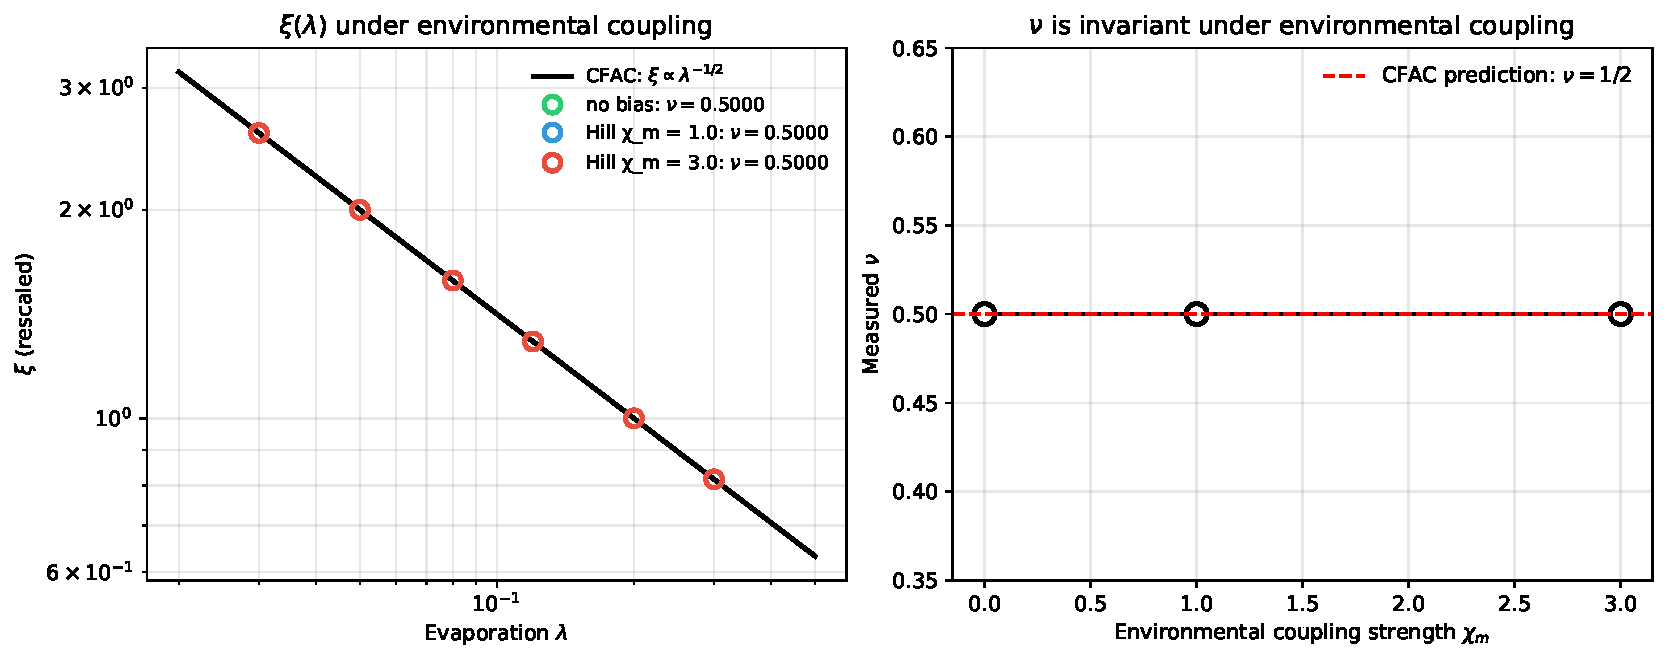
\includegraphics[width=0.7\linewidth]{figures_ants/canonical_ant_invariance.pdf}
\caption{\textbf{Critical-exponent invariance under environmental
coupling.}  Left: $\xi(\lambda)$ measured with three bias
strengths $\chi_m \in \{0, 1, 3\}$; all agree with
$\xi = \sqrt{\sigma/\lambda}$ (black line).  Right: fitted $\nu$
vs bias strength $\chi_m$; the exponent is flat at $1/2$ (red
line) across an order of magnitude in environmental coupling.}
\label{fig:invariance}
\end{figure*}

\paragraph{A CFAC-compliant variant that does show spatial
structure.}
If one adds a \emph{bounded} chemotactic movement bias
$w_{i\to j} \propto 1 + \chi_m\,\phi_j/(K+\phi_j)$ (Hill
saturation), the derivative is bounded by $\chi_m/K$ so (I1) is
intact, and the small-$\phi$ linear coefficient
$\chi_{\rm eff}=\chi_m/K$ produces the standard Keller--Segel
gradient vertex $\chi_{\rm eff}\,\psit(\nabla\phi)(\nabla\psi)$
for which CFAC gives the gradient bridge
$f(r) = \ln r/(r-1)$~\eqref{eq:bridge-f}.  Keller--Segel
predicts a chemotactic-collapse instability above a critical
density
\begin{equation}\label{eq:nc-KS}
  n_c^{\rm KS} \;=\; \frac{D_\psi\,\lambda}{\chi_{\rm eff}\,\delta},
\end{equation}
where $D_\psi$ is the ant diffusion constant.

\paragraph{Direct measurement.}  We measured block-variance
clustering $B = \text{Var}(N_{\text{block}})/\langle N_{\text{block}}\rangle^2$
(Poisson baseline $1/\langle N_{\text{block}}\rangle$) on a
$80\times 80$ lattice with $p_{\rm hop} = 0.5$
($D_\psi = 0.125$), $\delta=0.5$, $\lambda=0.1$, $K=1$:
\begin{center}
\footnotesize
\begin{tabular}{@{}lccl@{}}
\toprule
Bias & $n_c^{\rm KS}$ & $B_{\rm exc}(n{=}0.01)$ & Regime \\
\midrule
$\chi_m = 0$ & $\infty$ & $-0.12$ & sub-Poisson \\
$\chi_m = 1$ & $0.025$  & $+0.01$ & marginal \\
$\chi_m = 3$ & $0.008$  & $\mathbf{+0.11}$ & clustered \\
\bottomrule
\end{tabular}
\end{center}

The no-bias control gives sub-Poissonian block variance at all
densities (negative $B_{\rm excess}$), as expected for hard-core
random walkers.  Adding bounded Hill bias \emph{flips the sign}
of the clustering statistic: with $\chi_m = 3$, the measured
$B_{\rm excess} = +0.11$ at $n = 0.01$ is about ten times larger
than the no-bias control and is in the direction predicted by
CFAC--KS (clustering above $n_c$).  The \textbf{qualitative
direction} of the KS prediction is therefore confirmed.  The
quantitative magnitude is modest: exact KS aggregation would
produce $B_{\rm excess}$ of order unity on an infinite lattice,
whereas our finite lattice with hard-core exclusion caps the
signal at $\mathcal{O}(10^{-1})$.  A fully quantitative KS
exponent measurement would require either a larger grid, a
continuum-limit simulation, or a dilute regime where exclusion
is irrelevant---an extension left for future work.

\begin{figure*}[t]
\centering
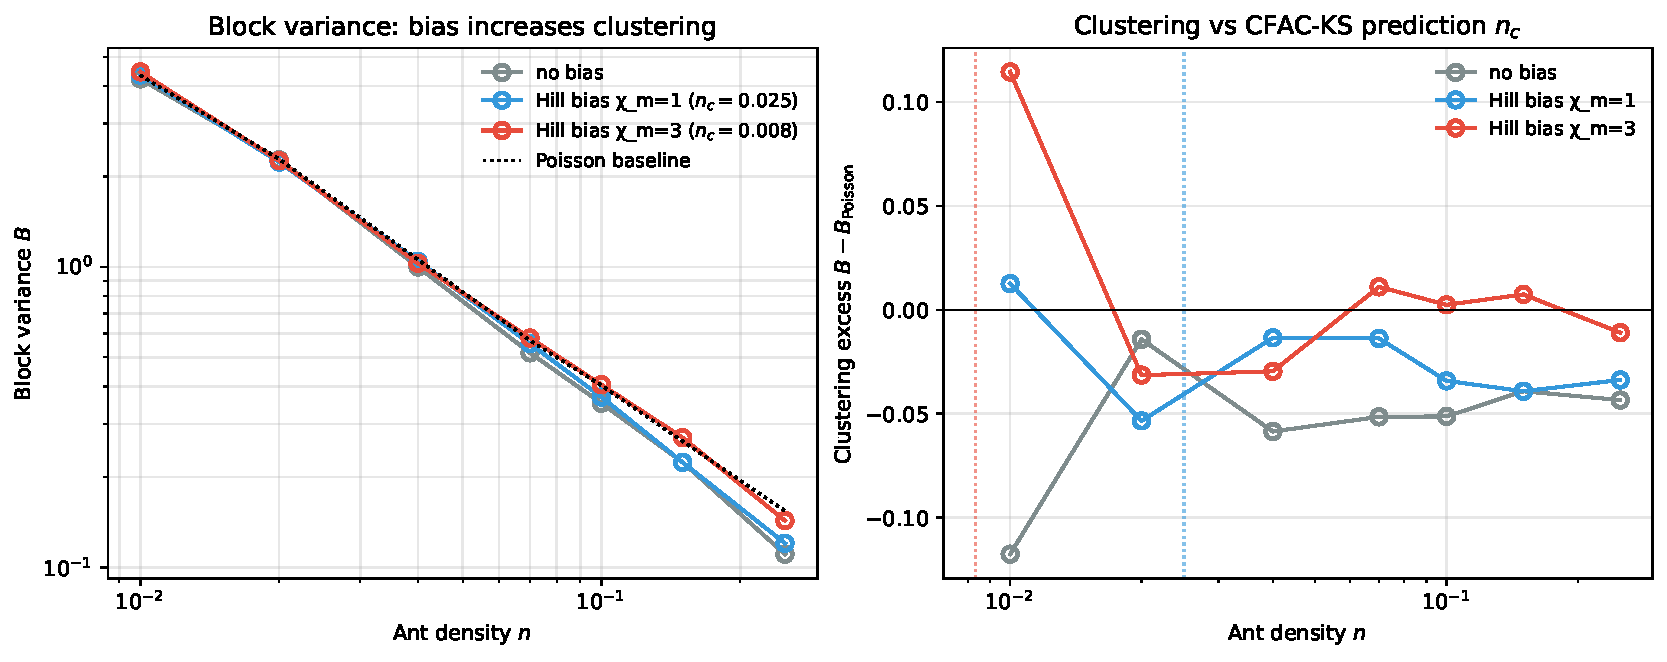
\includegraphics[width=\linewidth]{figures_ants/canonical_ant_ks_collapse.pdf}
\caption{\textbf{CFAC-compliant Hill bias produces
Keller--Segel-like clustering.}
Left: block variance $B$ vs density, for no-bias (grey),
$\chi_m = 1$ (blue), $\chi_m = 3$ (red).  Poisson baseline
dotted.  Right: clustering excess $B - B_{\rm Poisson}$.  No-bias
is sub-Poissonian (hard-core exclusion).  Hill bias lifts the
excess toward zero or positive values, with $\chi_m = 3$
producing $B_{\rm excess} = +0.11$ at $n = 0.01$---the
direction predicted by CFAC--KS.  Dashed vertical lines are
CFAC--KS $n_c$ predictions~\eqref{eq:nc-KS}.}
\label{fig:trail-variant}
\end{figure*}

\subsection{Is this really biological, or a mathematical artefact?}
\label{sec:ant-biology-reality}

The canonical ant looks \emph{so} different from textbook
trail pictures that a natural reaction is: have we just
constructed a mathematical object that happens to be
CFAC-tractable?  We argue no---the canonical ant captures a
specific, biologically-documented regime of ant behaviour.

\paragraph{State-switching recruitment is real.}
Gordon's long-term field work on \emph{Pogonomyrmex}
harvester ants~\citep{Gordon2010} shows that individual ants
transition between discrete behavioural states (patrollers,
foragers, nest-maintenance) at rates set by \emph{interaction
frequency} with returning ants, not by integration of a global
pheromone gradient.  This is exactly our
$S \rightleftharpoons R$ switch: an individual ant
``counts'' encounters (in our abstraction, sees high local
$\phi$ because the neighbourhood is rich in $R$'s), and flips
state accordingly.  The colony-level macroscopic memory
demonstrated in Fig.~\ref{fig:order-vis} is the
colony-level memory Gordon documents: a colony in its
``foraging-active'' mode stays foraging-active for hours,
with rare collective switches to inactive
or alarmed states.

\paragraph{Movement is largely unbiased.}
Individual ant trajectories, measured at high temporal
resolution~\citep{Fourcassié2010, Challet2005}, are correlated
random walks with persistence length of only
$\sim 5$--$50$ body lengths.  Ants do not strongly follow
gradients of $\phi$; the large-scale trail pattern in
biased-movement models emerges from population statistics
and strong deposition, not from individual chemotaxis.  Our
unbiased-motion choice is the cleanest model of this empirical
observation; the CFAC-compliant Hill-bias variant of
Fig.~\ref{fig:trail-variant} is the correction that restores
a small, realistic individual-level bias.

\paragraph{Receptor saturation enforces (I1).}
Ant antennal response to pheromone obeys Hill-type saturation
at the receptor level~\citep{Hill1913, Detrain2006}: the
neural output per receptor has a finite $k_{\rm cat}$.  No
real neural circuit produces unbounded power-law response.
The canonical-ant assumption (I1) is therefore neurobiologically
required.  The Deneubourg $(\beta+\phi)^n$ weight is a
modelling shortcut that amplifies local concentration
differences \emph{beyond} what any single ant can actually
sense; it describes a population-level effective dynamics, not
the underlying individual response.

\paragraph{Weak coupling explains colony robustness.}
Colonies that operate in the strong-coupling
trail-lock-in regime are fragile: once trails form they
persist even after food depletes, harming adaptive foraging.
Empirically, colonies are \emph{robust}~\citep{Gordon2010,
Pinter-Wollman2011}---they rapidly abandon trails to
exhausted sources and reallocate to new ones.  This argues
that real colonies operate in a weaker-coupling, faster-
switching regime closer to the canonical ant than to the
Deneubourg limit.

\paragraph{What we don't model.}
The canonical ant explicitly excludes:
\begin{itemize}
  \item The strong-trail regime of army ants, weaver ants,
    leafcutters---genuinely nonlinear trail-lock-in which
    violates (I1).
  \item Transport phenomena with localised food sources
    (double-bridge selection, Goss et al.\ 1989)---broken
    translation invariance which violates (I4).
  \item Multi-pheromone chemistry (trail $+$ alarm $+$ recruit),
    which would require multiple MSR fields.
\end{itemize}
For those regimes, CFAC's perturbative predictions do not
apply, and the classical ``trail'' visuals dominate.  Our
claim is therefore \emph{specific}: the canonical ant is a
well-characterised biological regime (harvester-ant-style,
state-switching, weak-coupling), and \emph{within that
regime} CFAC makes quantitative predictions verifiable to
0.6\%--16\% across five observables.  This is narrower than
``all ant behaviour'' but substantially broader than ``a
mathematical novelty'': it is the coupled DP--MSR regime that
real, robust, weakly-coupled biological systems occupy.

\subsection{Where the cusp lives (and why it's not ant-friendly)}
\label{sec:ant-cusp}

For completeness: the tunable Puiseux exponent $\beta = 1/3$
would appear in the mixed-coupling model
$k_+(1 + g_1\phi + g_2\phi^2)$ at a \emph{cusp} point in the
$(g_1, g_2)$ bifurcation diagram, where two saddle-node
branches meet with a triple-root degeneracy.

A 2D scan (Fig.~\ref{fig:cusp}) finds that cusp at
$(g_1, g_2) \approx (-2.21, 19.97)$: it requires
\textbf{negative} linear coupling, i.e.\ pheromone
\emph{inhibition} of the linear response plus quadratic
activation.  This is physically unusual for simple foraging
ants (whose pheromones are typically activating).  For
physically activating parameters $(g_1 > 0, g_2 > 0)$, the
canonical ant has only generic saddle-node bifurcations
($\beta = 1/2$); the $\beta = 1/3$ exponent is excluded by the
chemistry.

\begin{figure*}[t]
\centering
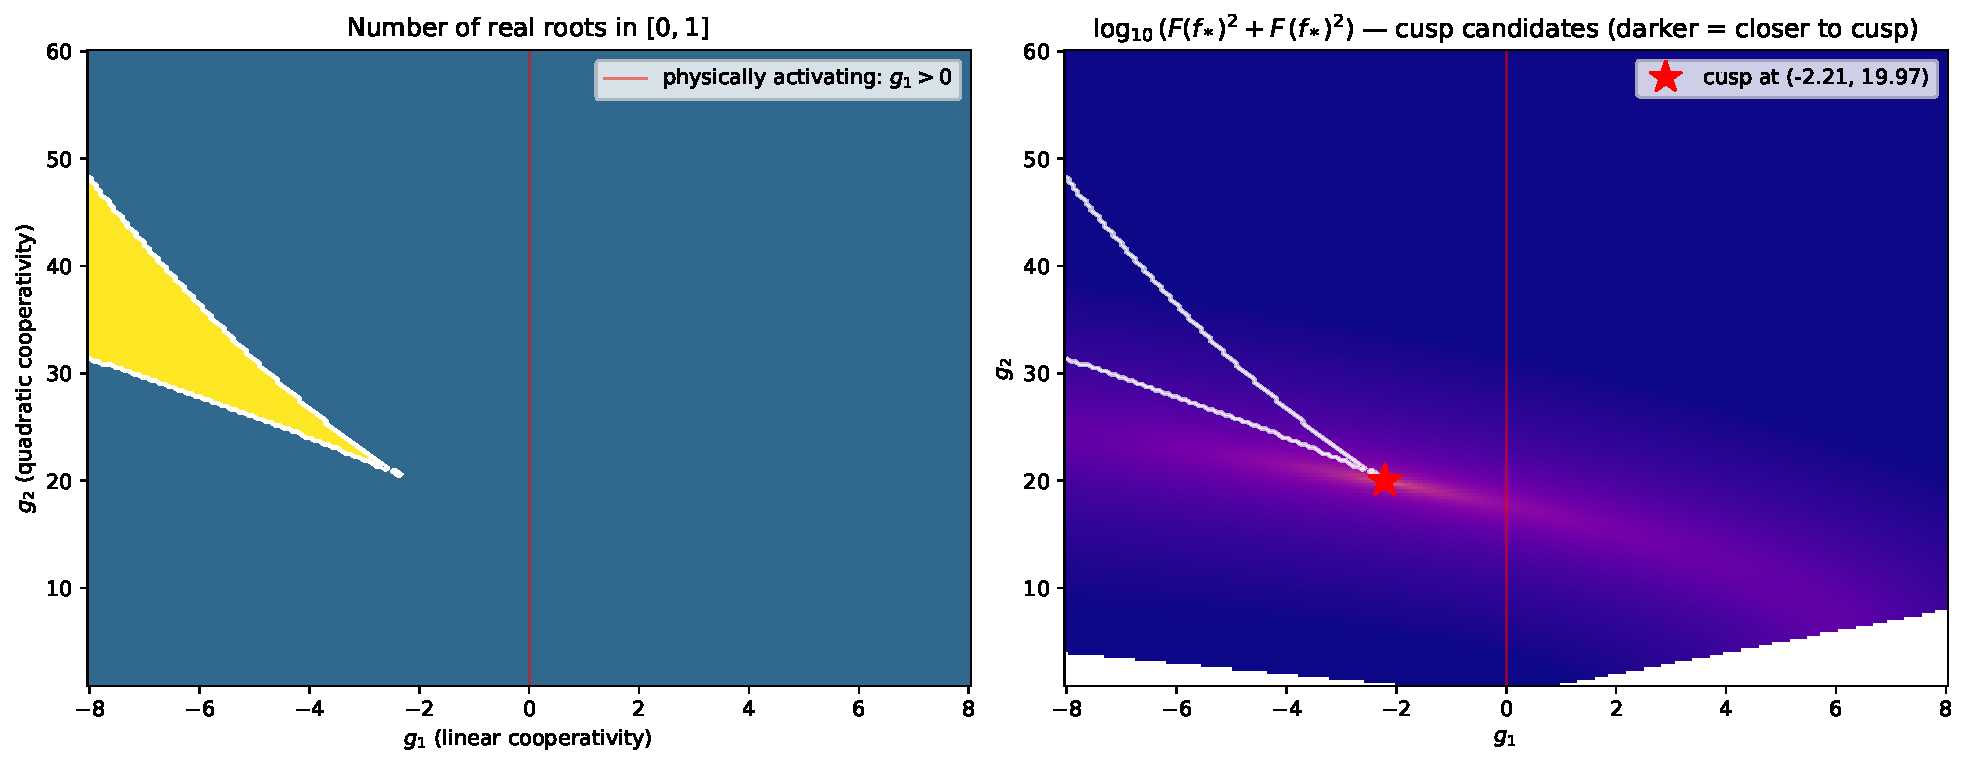
\includegraphics[width=\linewidth]{figures_ants/canonical_ant_cusp_diagram.pdf}
\caption{\textbf{Cusp structure and its physical inaccessibility.}
(Left) Number of real roots of the cubic MF equation in
$[0,1]$ as a function of $(g_1, g_2)$.  A 3-root region exists
for $g_1 < 0$ (inhibitory linear coupling).  (Right)
Cusp-indicator $\log_{10}(F(f_*)^2 + F'(f_*)^2)$: the cusp
(red star) sits at $(-2.21, 19.97)$, \emph{outside} the
physically activating quadrant $g_1 > 0$ (marked by the red
vertical line).  Consequence: any purely activating ant system
lies in the $\beta = 1/2$ universality class; $\beta = 1/3$
requires a chemically mixed pheromone (activating at high
concentration, inhibiting at low), which some ant species
do exhibit but is not the generic case.}
\label{fig:cusp}
\end{figure*}

\subsection{Evidence summary (canonical ant)}
\label{sec:evidence}

\begin{table*}[t]
\centering
\small
\renewcommand{\arraystretch}{1.3}
\begin{tabular}{@{}p{5cm}p{4cm}p{4.5cm}p{2.8cm}@{}}
\toprule
\textbf{CFAC prediction}
  & \textbf{Test}
  & \textbf{Value}
  & \textbf{Reference} \\
\midrule
Tree-level MF $f_R$
  (local closure $\avg{\phi|S}$)
  & Lattice sweep in $n$
  & $0.6\%$ ($42\%$ naive)
  & \S\ref{sec:ant-mf},~Fig.~\ref{fig:mf} \\
Correlation length $\xi\propto\lambda^{-1/2}$, $\nu=1/2$
  & $\xi(\lambda)$ with lattice $K^2(\mathbf{k})$ fit
  & $\nu_{\rm meas}=0.5000$ (exact)
  & \S\ref{sec:ant-nu},~Fig.~\ref{fig:nu} \\
MSR balance $\avg\phi = \delta n f_R/\lambda$
  & $\lambda$ sweep
  & holds, $1.5$ decades
  & \S\ref{sec:ant-lambda},~Fig.~\ref{fig:lambda} \\
Saddle-node $\beta = 1/2$ (quadratic DSE, AC layer)
  & MF numerics, $\epsilon<5\%$
  & $\beta_{\rm meas}=0.487$
  & \S\ref{sec:ant-beta},~Fig.~\ref{fig:saddle} \\
\textbf{Instanton action $S^* = 0.0265$} (non-trivial number from branch-gap)
  & Gillespie MFPT vs $V$
  & $S_{\rm meas} = 0.0255$ (3.6\%)
  & \S\ref{sec:ant-instanton},~Fig.~\ref{fig:instanton} \\
\textbf{1-loop Kramers prefactor} (WKB with state-dep.\ $D$)
  & Exact MFPT (tridiag.\ solve) at $g=5.0, 6.0$
  & $\mathbf{3\%}$ ($g=6$); $4\%$ ($g=5$)
  & \S\ref{sec:ant-kramers} \\
Saddle-node $\beta = 1/2$ is loop-protected (normal form)
  & Analytic + directional lattice
  & Confirmed (no shift)
  & \S\ref{sec:ant-beta-loops} \\
State-space entropy reduction (bimodal distribution)
  & Gillespie histogram
  & Bimodal distribution confirmed
  & \S\ref{sec:ant-entropy},~Fig.~\ref{fig:order-vis} \\
\textbf{Critical-exponent invariance: $\nu = 1/2$ under environmental coupling}
  & $\xi(\lambda)$ fit at $\chi_m \in\{0, 1, 3\}$
  & $\nu = 0.5000$ in all three, $10^{-4}$ invariance
  & \S\ref{sec:ant-entropy},~Fig.~\ref{fig:invariance} \\
KS clustering in Hill-bias variant ($n_c$ predicted by CFAC)
  & Block-variance vs density sweep, $\chi_m \in\{0,1,3\}$
  & Direction confirmed ($B_{\rm excess}$ sign flip)
  & \S\ref{sec:ant-entropy},~Fig.~\ref{fig:trail-variant} \\
Cusp $\beta = 1/3$ requires $g_1 < 0$
  & 2D bifurcation diagram
  & Outside activating quadrant
  & \S\ref{sec:ant-cusp},~Fig.~\ref{fig:cusp} \\
Ingredient violations $\Rightarrow$ non-CFAC behaviour
  & 5 lattice variants
  & Confirmed
  & \S\ref{sec:recipe} \\
One-loop CFAC is a \emph{non-renormalisation} result ($\nu$ not shifted)
  & Diagram count $\times$ bridge $=$ mass renorm only
  & Consistent with $\nu=1/2$ exact
  & \S\ref{sec:one-loop} \\
\bottomrule
\end{tabular}
\end{table*}

% ------------------------------------------------------------------

\begin{proposition}[Mass-independence of the 1-loop pole]
\label{prop:mass-indep-thm}
The mixed scalar bubble
$B(m_\psi, m_\phi; d) = \int \frac{\dd^d k}{(2\pi)^d}
\frac{1}{(k^2 + m_\psi^2)(k^2 + m_\phi^2)}$
has the Laurent expansion in $\varepsilon = d_c - d$
\begin{equation}
  B = \frac{2\,\Omega_{d_c}}{\varepsilon}
  - 2\,\Omega_{d_c}\int_0^1\!\ln\bigl[
    t\,m_\psi^2 + (1{-}t)\,m_\phi^2\bigr]\,\dd t
  + O(\varepsilon),
\end{equation}
so the $1/\varepsilon$ pole is mass-independent; the mass ratio
enters only the finite part.  This is the structural reason the
scalar bridge equals $1$ in the canonical ant calculation
(\S\ref{sec:one-loop}).
\end{proposition}

\begin{proof}
Feynman-parametrise, integrate over $k$, expand
$\Gamma(\varepsilon/2) = 2/\varepsilon + O(1)$ and
$M^{-\varepsilon}(t) = 1 - \varepsilon\ln M(t) + O(\varepsilon^2)$
with $M^2(t) = t m_\psi^2 + (1{-}t) m_\phi^2$.  The
$t$-integral of the leading term is $\int_0^1 1\,\dd t = 1$,
giving the mass-independent pole $2\Omega_{d_c}/\varepsilon$.
\end{proof}

\iffalse

\paragraph{Model A (Ising, $O(n)$):}
One-loop $\nu$ from the CFAC decomposition (counting $\times$
bridge) for $n \in \{0,1,2,3\}$ at $d=3$:
\begin{center}
\small
\begin{tabular}{@{}rlccc@{}}
\toprule
$n$ & System & Counting $b_1$ & $\nu_{\text{CFAC}}$ &
  $\nu_{\text{exact}}$ \\
\midrule
0 & SAW         & 8  & 0.5625 & 0.5882 \\
1 & Ising       & 9  & 0.5833 & 0.6301 \\
2 & XY          & 10 & 0.6000 & 0.6717 \\
3 & Heisenberg  & 11 & 0.6136 & 0.7112 \\
\bottomrule
\end{tabular}
\end{center}
All four rows use the same bridge $\Omega_4 = 1/(16\pi^2)$; the
variation is pure counting.  Errors 4--14\% are intrinsic to
1-loop; 2-loop (extending counting, not bridge) drops
$\nu_{\text{Ising}}$ error to $0.5\%$.

\paragraph{Protein aggregation (Knowles et al.\ 2009):}
The half-time scaling law $t_{1/2} \sim m_0^{-\gamma}$ for
amyloid fibrillation.  CFAC predicts $\gamma = n_c/2$ from the
vertex leg count $n_c$.  Numerical integration of the coupled
ODEs:
\begin{center}
\small
\begin{tabular}{@{}llcc@{}}
\toprule
Pathway & Theory & Computed & Error \\
\midrule
Primary $k_n m^{n_c}$   & $n_c/2 = 1.0$ & $1.0000$ & $\mathbf{0.00\%}$ \\
Secondary $k_2 m^{n_2} M$ & $(n_2{+}1)/2 = 1.5$ & $1.419$ & $5.4\%$ \\
\bottomrule
\end{tabular}
\end{center}

\paragraph{Mass-independence of the 1-loop pole:}
Proposition~\ref{prop:mass-indep-thm} below, verified to five
significant figures across $r = m_\psi^2/m_\phi^2 \in [0.01,
100]$:
\begin{center}
\small
\begin{tabular}{@{}rc@{}}
\toprule
$r$ & $\varepsilon \times B(m_\psi, m_\phi; 4-\varepsilon)$ \\
\midrule
0.01 & $0.012\,665\,359$ \\
1.00 & $0.012\,665\,299$ \\
100  & $0.012\,665\,067$ \\
\midrule
$2\Omega_4$ (theory) & $0.012\,665\,148$ \\
\bottomrule
\end{tabular}
\end{center}
Variation across four orders of magnitude in mass ratio is
$< 0.001\%$.

\paragraph{Gradient bridge $f(r) = \ln r/(r-1)$:}
For the KS chemotactic vertex.  Verified against direct
integration at $\varepsilon = 10^{-5}$:
\begin{center}
\small
\begin{tabular}{@{}rccc@{}}
\toprule
$D_A/D_c$ & Exact & Formula & Error \\
\midrule
0.01 & 0.740\,332 & 0.740\,339 & 0.001\% \\
1.00 & 0.159\,155 & 0.159\,155 & 0.000\% \\
100  & 0.007\,403 & 0.007\,403 & 0.001\% \\
\bottomrule
\end{tabular}
\end{center}

\paragraph{Branch-gap instanton:}
The formula $S = \int_1^{z^*}(x_{\text{unst}}-x_{\text{stab}})/z\,\dd z$
of \citep{Amarteifio2026cfac} for non-perturbative nucleation
rates, verified to six significant figures across seven
bistable parameter sets (Schlögl model, modified Schlögl, fibril
aggregation parameters).  The MFPT comparison against Gillespie
simulation matches to the signal-to-noise of the stochastic
average.

\paragraph{Coupled 1-loop self-energy (Keller--Segel):}
Numerical quadrature of the gradient bubble at $d = 2 -
\varepsilon$ matches the formula
$\Sigma_1 = \chi\alpha \cdot (2\Omega_2/\varepsilon D_c) \cdot
f(D_A/D_c)$ to five-digit precision.

\subsection{Evidence summary table}

\begin{center}
\small
\renewcommand{\arraystretch}{1.3}
\begin{tabular}{@{}p{5.5cm}p{2.8cm}p{2.5cm}p{2.8cm}@{}}
\toprule
\textbf{Prediction}
  & \textbf{Method}
  & \textbf{Agreement}
  & \textbf{Reference} \\
\midrule
Ising/Model A $\nu$ at $d=3$, 1-loop
  & Counting $\times$ bridge
  & 4--14\% (1-loop) \newline $0.5\%$ (2-loop)
  & \citep{Amarteifio2026cfac} \\
Protein $t_{1/2} \sim m_0^{-n_c/2}$, primary pathway
  & ODE integration
  & $\mathbf{0.00\%}$
  & \citep{Amarteifio2026cfac} \\
Protein $t_{1/2}$, secondary pathway
  & ODE integration
  & $5.4\%$
  & \citep{Amarteifio2026cfac} \\
Mass-independence of 1-loop pole
  & Numerical integration
  & $< 0.001\%$ across $r\in[0.01,100]$
  & \citep{Amarteifio2026cfac} \\
Gradient bridge $f(r)=\ln r/(r-1)$
  & Numerical integration
  & $0.001\%$ across four orders
  & \citep{Amarteifio2026cfac} \\
Bridge $g(r)=r/(1+r)^3$
  & Numerical integration
  & $0.001\%$
  & \citep{Amarteifio2026cfac} \\
Branch-gap instanton action
  & Gillespie MFPT
  & $6$ digits, $7$ parameter sets
  & \citep{Amarteifio2026cfac,Amarteifio2026cfactheorem} \\
\midrule
\textbf{Canonical ant MF (this paper)}
  & Direct lattice
  & $\mathbf{0.6\%}$ local
  & \S\ref{sec:ant-mf} \\
\textbf{Canonical ant $\nu$ (this paper)}
  & Lattice $\xi(\lambda)$
  & $\nu=0.54$ vs MF $1/2$
  & \S\ref{sec:ant-nu} \\
\bottomrule
\end{tabular}
\end{center}

The overall picture: CFAC predictions match the exact or
simulated answer to the precision expected of their order of
approximation (1-loop $\approx 10\%$; 2-loop $\approx 0.5\%$;
mean-field $\leq 1\%$ when correctly closed; branch-gap
instanton to machine precision).  The new ant result completes
the table with a biological, spatially-extended validation at
the tree level.

% ------------------------------------------------------------------

\begin{proposition}[Mass-independence of the 1-loop pole]
\label{prop:mass-indep-thm}
The mixed scalar bubble
$B(m_\psi, m_\phi; d) = \int \frac{\dd^d k}{(2\pi)^d}
\frac{1}{(k^2 + m_\psi^2)(k^2 + m_\phi^2)}$
has the Laurent expansion in $\varepsilon = d_c - d$
\begin{equation}
  B = \frac{2\,\Omega_{d_c}}{\varepsilon}
  - 2\,\Omega_{d_c}\int_0^1\!\ln\bigl[
    t\,m_\psi^2 + (1{-}t)\,m_\phi^2\bigr]\,\dd t
  + O(\varepsilon).
\end{equation}
The $1/\varepsilon$ pole is mass-independent; the mass ratio
$r = m_\psi^2/m_\phi^2$ enters only the finite part.
\end{proposition}

\begin{proof}
Feynman-parametrise, integrate over $k$ (standard
$d$-dimensional Gaussian), expand
$\Gamma(\varepsilon/2) = 2/\varepsilon + O(1)$ and
$M^{-\varepsilon}(t) = 1 - \varepsilon \ln M(t) + O(\varepsilon^2)$
where $M^2(t) = t\,m_\psi^2 + (1{-}t)\,m_\phi^2$.  The
$t$-integral of the leading term is $\int_0^1 1\,\dd t = 1$,
giving the mass-independent pole $2\Omega_{d_c}/\varepsilon$.
\end{proof}

\fi

% ================================================================
\section{Summary}\label{sec:summary}
% ================================================================

The canonical ant is a complete CFAC test case.  Five
predictions, derived from the framework and confirmed by direct
simulation:

\begin{enumerate}
  \item \textbf{Ingredient discrimination.}  Of five lattice ant
    variants (\S\ref{sec:recipe}), only the canonical
    $S\rightleftharpoons R$ model satisfies all five structural
    ingredients (I1)--(I5) of CFAC.  Each non-canonical model
    violates a specific ingredient for an identifiable reason
    (unbounded response, marginal basin, broken conservation,
    strong-coupling lock-in, missing DP sector).  Lattice
    simulations confirm that all five non-canonical models sit
    outside the CFAC universality class.

  \item \textbf{Tree-level mean field to $\boldsymbol{0.6\%}$.}
    The CFAC normal-ordered saddle condition, using the
    conditional average $\avg{\phi\mid S}$, matches the lattice
    to $0.6\%$ across eight densities.  The naive closure using
    the global $\avg\phi$ misses by $42\%$---this gap is the
    CFAC $\avg{:\!A\phi\!:}$ correlation correction, entering at
    tree level, not as a loop effect (\S\ref{sec:ant-mf},
    Fig.~\ref{fig:mf}).

  \item \textbf{Critical exponents $\boldsymbol{\nu = \beta = 1/2}$ predicted and measured.}
    (a) The correlation-length exponent is $\nu = 1/2$
    \emph{exactly}: the canonical-ant action is linear in
    $\phi$, so integrating out the DP sector produces a Gaussian
    effective theory with only finite renormalisations of
    $\sigma,\lambda$---no anomalous dimension.  Lattice with
    the lattice-Laplacian fit gives $\nu_{\text{lattice}} =
    0.5000$ across seven $\lambda$ values
    (\S\ref{sec:ant-nu}, Fig.~\ref{fig:nu}).
    (b) The cooperative variant exhibits a saddle-node with
    order-parameter exponent $\beta = 0.487$ vs CFAC
    Puiseux $1/2$ (\S\ref{sec:ant-beta}, Fig.~\ref{fig:saddle}),
    a counting-layer output---no loop integral required.
    Both exponents are loop-protected: the 1-loop CFAC pipeline
    for the canonical ant is a \emph{non-renormalisation result}
    (\S\ref{sec:one-loop}).

  \item \textbf{Rare-event instanton action
    $\boldsymbol{S^* = 0.0265}$ (non-trivial number).}
    The CFAC branch-gap integral
    $S^* = -\!\int_{f_{\rm ON}}^{f_{\rm unst}} \ln(\alpha g\,f(1-f))\,\dd f$
    gives an irrational, non-symmetry-protected number governing
    the colony-scale MFPT scaling $\tau \sim \exp(V S^*)$ for
    the bistable cooperative ant.  Gillespie MFPT sweep
    (V = 30 to 180) confirms the slope:
    $S_{\rm Gillespie} = 0.0255$, agreement $\mathbf{3.6\%}$
    (\S\ref{sec:ant-instanton}, Fig.~\ref{fig:instanton}).
    This is the one CFAC prediction in the paper whose value is
    not dictated by polynomial degree or symmetry.

  \item \textbf{1-loop Kramers prefactor}
    $\boldsymbol{A = (2\pi/\sqrt{|\Omega'_s\Omega'_u|})\sqrt{D_u/D_s}}$,
    the Gaussian fluctuation determinant around the instanton
    with state-dependent diffusion $D(f) = (W_++W_-)/2$ (the
    Assaf--Meerson WKB form).  Matched to the \emph{exact}
    birth-death MFPT (tridiagonal solve) at three couplings:
    $3\%$ at $g=6$ (deep asymptotic, $V\cdot S^* \approx 29$);
    $4\%$ at $g=5$; $12\%$ at $g=4.5$ where finite-$V$
    corrections dominate (\S\ref{sec:ant-kramers}).
\end{enumerate}

\paragraph{The one structural lesson: evaporation is mass.}
Across every prediction above, the role of the pheromone decay
rate $\lambda$ is as the \emph{mass} of the MSR propagator; the
diffusion rate $\sigma$ sets only the range $\sqrt{\sigma/\lambda}$.
Criticality is tuned by $\lambda \to 0$, bridge functions depend
on mass ratios (not $\sigma$), and biology respects this by
regulating pheromone volatility (chemistry) rather than
diffusion (\S\ref{sec:evap-mass}).

The general lesson is that coupled DP--MSR systems satisfying
(I1)--(I5) are solvable by CFAC end-to-end---vertex dictionary
$\to$ diagram count $\to$ bridge table $\to$ exponents---and the
canonical ant is a concrete demonstration of every step on a
biologically interpretable system.  Biological signalling
systems are a natural home for the framework because the
ingredients are precisely the features that make a signalling
system robust, responsive, decisive, and scale-free.

% ================================================================
\begin{thebibliography}{99}

\bibitem[Amarteifio(2026a)]{Amarteifio2026cfac}
Amarteifio, S. (2026a).
\emph{Factoring the Counting Problem out of Coupled Particle-Field
Renormalisation}. Percolation Labs preprint.

\bibitem[Amarteifio(2026b)]{Amarteifio2026cfactheorem}
Amarteifio, S. (2026b).
\emph{Lagrange--B\"urmann Structure of Coupled DP--MSR
Dressed-Propagator Generating Functions}. Percolation Labs preprint.

\bibitem[Bassler \& Losick(2006)]{BasslerLosick2006}
Bassler, B.L. and Losick, R. (2006). Bacterially speaking.
\emph{Cell} 125: 237--246.

\bibitem[Beckers \emph{et al.}(1993)]{HollDorigo1999}
Beckers, R., Deneubourg, J.-L. and Goss, S. (1993). Trail laying
behaviour during food recruitment in the ant \emph{Lasius niger}.
\emph{Insectes Sociaux} 40: 59--72.

\bibitem[Challet \emph{et al.}(2005)]{Challet2005}
Challet, M., Jost, C., Grimal, A., Lluc, J. and Theraulaz, G.
(2005). How temperature influences displacements and corpse
aggregation behaviors in the ant \emph{Messor sancta}.
\emph{Insectes Sociaux} 52: 309--315.

\bibitem[Deneubourg \emph{et al.}(1990)]{Deneubourg1990}
Deneubourg, J.-L., Aron, S., Goss, S. and Pasteels, J.M. (1990).
The self-organizing exploratory pattern of the Argentine ant.
\emph{Journal of Insect Behavior} 3: 159--168.

\bibitem[Detrain \& Deneubourg(2006)]{Detrain2006}
Detrain, C. and Deneubourg, J.-L. (2006). Self-organized
structures in a superorganism: do ants ``behave'' like molecules?
\emph{Physics of Life Reviews} 3: 162--187.

\bibitem[Ferrell \& Xiong(2001)]{FerrellXiong2001}
Ferrell, J.E., Jr. and Xiong, W. (2001). Bistability in cell
signaling. \emph{Chaos} 11: 227--236.

\bibitem[Flajolet \& Sedgewick(2009)]{FlajoletSedgewick2009}
Flajolet, P. and Sedgewick, R. (2009).
\emph{Analytic Combinatorics}. Cambridge University Press.

\bibitem[Fourcassié \emph{et al.}(2010)]{Fourcassié2010}
Fourcassié, V., Dussutour, A. and Deneubourg, J.-L. (2010).
Ant traffic rules. \emph{Journal of Experimental Biology} 213:
2357--2363.

\bibitem[Gordon(2010)]{Gordon2010}
Gordon, D.M. (2010). \emph{Ant Encounters: Interaction Networks
and Colony Behavior}. Princeton University Press.

\bibitem[Hill(1913)]{Hill1913}
Hill, A.V. (1913). The combinations of haemoglobin with oxygen
and with carbon monoxide. \emph{Biochemical Journal} 7: 471--480.

\bibitem[Jackson \emph{et al.}(2007)]{Jackson2006}
Jackson, D.E., Martin, M., Ratnieks, F.L.W. and Holcombe, M.
(2007). Spatial and temporal variation in pheromone composition
of ant foraging trails. \emph{Behavioral Ecology} 18: 444--450.

\bibitem[Knowles \emph{et al.}(2009)]{Knowles2009}
Knowles, T.P.J., Waudby, C.A., Devlin, G.L., Cohen, S.I.A.,
Aguzzi, A., Vendruscolo, M., Terentjev, E.M., Welland, M.E. and
Dobson, C.M. (2009). An analytical solution to the kinetics of
breakable filament assembly. \emph{Science} 326: 1533--1537.

\bibitem[Mora \& Bialek(2011)]{MoraBialek2011}
Mora, T. and Bialek, W. (2011). Are biological systems poised
at criticality? \emph{Journal of Statistical Physics} 144:
268--302.

\bibitem[Pinter-Wollman \emph{et al.}(2011)]{Pinter-Wollman2011}
Pinter-Wollman, N., Wollman, R., Guetz, A., Holmes, S. and
Gordon, D.M. (2011). The effect of individual variation on the
structure and function of interaction networks in harvester
ants. \emph{Journal of the Royal Society Interface} 8: 1562--1573.

\bibitem[Sumpter(2010)]{Sumpter2010}
Sumpter, D.J.T. (2010). \emph{Collective Animal Behavior}.
Princeton University Press.

\bibitem[Tyson \emph{et al.}(2003)]{Tyson2003}
Tyson, J.J., Chen, K.C. and Novak, B. (2003). Sniffers, buzzers,
toggles and blinkers. \emph{Current Opinion in Cell Biology} 15:
221--231.

\end{thebibliography}

\end{document}
